\documentclass{suepthesis}

\SUEPSetup{
  cover = {
    date = 2026年5月7日,
  },
  info = {
    title = 基于云原生与 AI 辅助的,
    subtitle = 一体化在线编程评测平台设计与实现,
    titleEn = {Design and Implementation of an Integrated Online Programming Evaluation Platform Based on Cloud Native and AI Assistance},
    institution = 人工智能学院,
    major = 计算机科学与技术专业,
    author = 陆卡里,
    studentId = 20221499,
    supervisor = 范自柱,
    keywords = {在线编程评测平台；云原生；容器化判题；人工智能辅助；程序设计教学},
    keywordsEn = {online programming evaluation platform; cloud native; containerized judging; AI-assisted feedback; programming education},
  }
}

\usepackage[
  backend=biber,
  style=gb7714-2015,
  gbalign=gb7714-2015,
  gbnamefmt=lowercase,
  gbpub=false,
  sorting=none
]{biblatex}
\addbibresource{content/thesis.bib}

\usepackage[perpage,bottom,hang]{footmisc}
\graphicspath{{figures/}{images/}}
\DeclareGraphicsExtensions{.pdf,.eps,.png,.jpg,.jpeg}
\usepackage{booktabs}
\usepackage{multirow}
\usepackage{dcolumn}
\usepackage{placeins}
\usepackage{etoolbox}
\preto{\subsection}{\FloatBarrier}
\usepackage{ragged2e}
\usepackage{xltabular}
\keepXColumns
\newcolumntype{d}[1]{D{.}{.}{#1}}
\newcolumntype{P}[1]{>{\raggedright\arraybackslash}p{#1}}
\usepackage{longtable}
\setlength{\LTcapwidth}{\textwidth}
\usepackage{threeparttable}
\usepackage{threeparttablex}
\usepackage[ruled,vlined,linesnumbered]{algorithm2e}
\usepackage{siunitx}[=v2]
\usepackage{tikz}
\usetikzlibrary{arrows.meta, positioning, shapes.geometric, automata, calc, fit, backgrounds}
\usepackage{hologo}
\usepackage{minted}
\usepackage{verbatim}
\usepackage{xurl}
\providecommand{\dd}{\mathop{}\!\mathrm{d}}
\providecommand{\ee}{\mathrm{e}}
\providecommand{\ii}{\mathrm{i}}
\providecommand{\jj}{\mathrm{j}}
\providecommand{\XeTeX}{\hologo{XeTeX}}
\providecommand{\BibLaTeX}{\textsc{Bib}\LaTeX}
\DeclareRobustCommand\cs[1]{\texttt{\char`\\#1}}
\providecommand\pkg[1]{{\sffamily#1}}
\newcommand{\todoboxfigure}[2]{%
  \begin{figure}[htbp]
    \centering
    \fbox{\parbox{0.88\textwidth}{\small #2}}
    \caption{#1}
  \end{figure}%
}
\sloppy

\begin{document}
\MakeCover
\MakeOriginality
\frontmatter
\begin{abstract}

在数字化教育快速发展的背景下，课程电子化与教学互联网化日益普及，本科程序设计课程中的一体化在线评测平台便是数字化浪潮中的重要产物。然而，现有平台在实际教学中存在着一常见问题：学生提交代码后只能看到最终判题结论，例如“答案错误”或“编译错误”，无法判断失败是发生在排队、编译还是运行阶段；同时平台开发方又不得不在安全隔离、并发处理能力与反馈可解释性之间做出工程妥协。针对上述问题，本文设计并实现了一个面向本科程序设计课程的一体化在线评测平台。该系统将客观判题作为主干，AI分析只做辅助，两者之间通过数据交换联系，但不共用流程，从而保证判题结果的稳定性不受AI模块波动的影响。

本系统的判题流程将提交受理和执行分开处理。用户提交代码时，系统先创建一条状态为排队中的记录，同时投递一个 Inngest 事件。后台函数准备 Docker 容器、上传源码、完成编译、按测试用例逐一运行并清理现场。执行过程放在受控的 Docker 沙箱内，并设置了内存上限和网络隔离。状态变化通过 Soketi 实时推送到前端，避免轮询。为便于排查问题，数据层没有只存最终结果，而是拆成三个模型：Submission 存放提交的基本信息，Judge 记录本次判题的整体状态，JudgeRun 保存每个测试用例的输入、输出、消耗时间和内存。

本系统还围绕代码提交的前后环节给出教学方面的支持，提交之前，系统利用 Monaco 编辑器还有容器化 Clangd 服务给出代码补全、语法诊断还有函数签名提示功能；提交之后，AI 模块会异步生成复杂度、代码风格、可读性、运行效率以及正确性等内容的分析结果，还会把这些分析结果跟客观判题结果分开储存。验证结果表明，系统可以稳定处理正确通过、编译错误、答案错误、运行时错误、超时以及内存超限这些常见情况，还能借助资源限制和网络隔离阻挡恶意提交。跟只给出最终判题结论的传统平台相比，本系统更符合本科程序设计教学的实际需求。

\end{abstract}

\begin{abstractEn}

This paper implements an integrated online evaluation platform for undergraduate programming teaching scenarios. The starting point of the topic selection comes from the actual teaching pain points : students often can only see the final judgment state, and it is difficult to judge whether the failure occurs in the queuing, compiling or running stage, while the platform side needs to make engineering choices between security isolation, concurrent processing and feedback interpretability. In response to these problems, this paper takes objective judgment as the core process, and AI ability as an independent teaching assistant process, which is decoupled from the judgment process to ensure the stability and certainty of the judgment process.

This paper adopts the decoupling scheme of submission acceptance and asynchronous execution in the judgment process. The submission entry first creates a record with a state of QD and delivers the Inngest event. The background function completes the container preparation, source code upload, compilation, run and clean up one by one according to the test case. The  execution phase runs in a controlled Docker sandbox, and combines memory constraints and network isolation to guarantee execution boundaries. The state change is transmitted back to the front end in real time through the Soketi channel to reduce the polling overhead. In order to improve the traceability, the data layer divides the judgment information into three layers : Submission, Judge and JudgeRun, which respectively carry the submission summary, the main state of the judgment and the execution track of each test case, so as to completely record the whole process of the judgment process from acceptance to final state.

On the teaching support side, the platform covers support capabilities in two stages, before and after submission. Before submission, the front-end workspace integrates Monaco with Language Server Protocol to provide completion, diagnostics, and signature help through containerized Clangd. After submission, the AI module asynchronously generates multi-dimensional analysis results, including complexity, comprehensive score, code style, readability, efficiency, and correctness, and provides executable improvement suggestions. The analysis results are stored separately from objective judgment results to avoid the interpretation module affecting the certainty of the ruling. The system supports Chinese and English interface and topic switching, and the AI analysis text can output Chinese or English feedback according to the current language environment. Verification results show that the platform can stably complete AC, CE, WA, RE, TLE, and MLE core state determination, and the asynchronous link and real-time state push can work continuously. In response to malicious samples such as \texttt{fork()} abuse, oversized memory requests, and network outreach requests, the system can also block risky behavior under resource restriction and network isolation strategies. Compared with the traditional teaching OJ represented by UOJ, which mainly focuses on the final verdict, this system provides integrated capabilities of semantic diagnosis before submission, real-time state visualization during submission, and multi-dimensional interpretation feedback after submission while maintaining the stability of objective judgment, reflecting system features and engineering innovation oriented to teaching process support.

\end{abstractEn}

\MakeTOC
\mainmatter
\chapter{绪论}

\section{研究背景及意义}

随着信息技术、工程教育改革、在线教学模式的不断发展，程序设计类课程对高校人才培养模式中的作用越来越显著。程序设计教学不仅要求学生掌握语法知识，还要求其拥有算法设计、问题抽象、调试分析和工程实现能力。如何在大规模教学场景中达成高效率、客观化且可重复的程序作业评价就成为了计算机类课程建设的关键问题之一，而在线编程评测平台的出现，为这一问题提供了较为有效的解决路径，在线编程评测平台借助自动编译、运行、测试用例比对、结果反馈等机制给程序设计教学予以了标准化支持，显示出较高的教学应用价值\cite{kurnia2001online,leal2003mooshak,ala2005survey}。

传统的在线编程评测平台大多只围绕提交即判分这一基本模式展开，虽然这样能够完成结果判定，但在教学反馈、资源弹性和平台运维等方面存在明显短板。一方面，单体式系统在高并发提交场景下容易受到资源瓶颈影响，另一方面，学生在面对编译错误、运行错误或答案错误时只能获得较为简短的判题结论，难以快速定位问题原因。对于以过程性学习和能力培养的教学场景而言，仅依赖传统的评测逻辑已难以满足更高层次的系统设计需求\cite{ala2005survey,keuning2018feedback,barczak2023automated}。

与此同时，云原生、容器化和微服务架构的快速发展为评测平台提供了更具可操作的技术路径。判题任务在教学场景里经常呈现出短时高峰、语言环境差异大、隔离要求严格等特征，这些特征与容器执行、服务拆分、弹性调度天然契合\cite{burns2016borg,balalaie2016microservices,difrancesco2019microservices,hezhenwei2020kubernetes}。将这些技术引用到系统中的价值并不仅限于部署到云上，还在于提升判题环境一致性、扩展弹性和长期维护可控性。

近年来，大语言模型和代码智能技术的发展又让在线评测平台具备了进一步提升反馈质量的可能。传统平台大多只能返回 \texttt{AC}、\texttt{WA}、\texttt{CE} 等简短状态，而实际应用场景中学生真正关心的是代码错在哪里、为什么会错以及应该怎么修改。在这方面，AI 技术就适合承担解释和提示的作用，但是不适合直接让 AI 进行判题或替代判题的主体\cite{keuning2018feedback,sarsa2022llm,jacobs2024feedback,wangfang2023ai,zhanghongzhuo2024genai}，如何在保证判题公平的前提下合理接入 AI 辅助反馈机制正是本文关注的重要问题之一。

基于上述背景，本文选择在线编程评测平台作为研究对象，并尝试在其中引入云原生执行环境与 AI 辅助反馈两类技术手段来解决两个较为实际的问题，如何将自动判题平台做得更稳定、更安全、更便于扩展以及如何在不影响判题公平性的前提下为学生补充更有用的解释性反馈。

\section{国内外研究现状}

综合上述工作可以看到，自动评测研究已经回答了如何保证判题正确与可重复，云原生研究提供了如何支撑弹性执行与资源约束，AI 教育研究则扩展了如何生成更具解释性的学习反馈。问题在于，这三类成果往往在不同系统中各自推进。面向评测业务的并发调度细节，常被云侧通用框架弱化，AI 反馈也常作为外挂能力存在，难以和判题流程共享上下文。本文的切入点正是缩小这三者之间的工程断层。

国外学者于自动判题、在线编程评测领域收获了诸多成果。Kurnia 等人讲述了 Online Judge 系统的设计运行状况，证明自动评测在大规模教学与训练场景具备可行性\cite{kurnia2001online}，Leal 和 Silva 所提出的 Mooshak 系统让竞赛与课程场景下的题目组织、提交流程、结果反馈机制更为规范\cite{leal2003mooshak}。Ala-Mutka 在自动评测方法综述当中，从功能正确性、效率、风格等多个方面对评估方法予以了比较全面的梳理\cite{ala2005survey}，Ihantola 等人在程序作业自动评估综述里剖析了自动反馈与教学场景的关系\cite{ihantola2011automated}，Keuning 等人又做了进一步说明。过程性、解释性反馈对学生学习编程有着不小的帮助，不过许多平台在反馈方面的程度仍有进步空间\cite{keuning2018feedback}。Paiva 等人在针对计算机科学作业的自动评测综述里观察到，效率、行为还有可读性等维度不断进入评估范围，容器化和静态分析技术助力评测平台的工程形态变得更完善\cite{paiva2022automated}。Messer 等人经过系统综述总结了自动评分与反馈工具的研究热点，表明评测维度、自动化程度、评估方法之间不均衡情况显著，公开数据集不足同样限制了不同工具之间的横向比较\cite{messer2024automated}。Barczak 等人在最新综述中归纳了自动评测平台的多条技术路线\cite{barczak2023automated}。

在云原生、容器化这一领域，Burns 等人针对 Borg 等大规模集群管理系统展开总结，其结果显示，容器编排、统一调度机制在应对短时突然出现的负载、实现资源的共享、多节点之间的协同工作这些方面，具备显著优势\cite{burns2016borg}，Balalaie、Di Francesco 等人围绕微服务架构、实证分析做了进一步阐述，他们指出，依据业务职责对模块进行拆分，对于独立部署、独立演化、故障隔离而言，有着积极的意义\cite{balalaie2016microservices,difrancesco2019microservices}，Docker 与 Kubernetes 的官方文档，还有 NIST 容器安全指南，从工程实践、安全规范这两个方面，为容器化的执行提供了相对完整的参考\cite{dockerdocs,kubernetesdocs,nist201716800190}。在 AI 辅助编程反馈这一方向上，Sarsa 等人探索了借助大语言模型来生成编程练习、代码解释的可行性\cite{sarsa2022llm}，Jacobs 等人对大语言模型自动反馈在入门编程课程里的实际效果做了评估\cite{jacobs2024feedback}。Finnie-Ansley 等人进行了关于 Codex 在入门编程教学中影响的研究，指出代码生成模型可能会改变学生练习和考核的形态，所以要重新审视学术诚信、能力培养目标\cite{finnieansley2022robots}，Denny 等人通过 Copilot 提示工程实验，发现自然语言与代码协同交互正在形成新的学习路径\cite{denny2023conversing}，Kazemitabaar 等人的实验研究表明，AI 代码生成器在提高新手提示效率的时候也可能会引发过度依赖\cite{kazemitabaar2023chi}。Raihan 等人通过系统文献综述梳理了大语言模型进入计算机教育的多条路径，包括课程建设、学习支持与风险治理等方向\cite{raihan2025llmcsed}，Koutcheme 等人证实开源大模型在生成反馈、作为评判者去评估反馈质量这两项任务方面有着实际潜力\cite{koutcheme2024evaluatinglm,koutcheme2024openfeedbackiticse}，Lubin 等人探讨了大语言模型在编程教学中的能力界限、使用规范\cite{lubin2025llm}。

国内研究起步相对略晚，但近年来在 OJ 平台、容器化教学环境与 AI 辅助教学等方面均有较快推进。Tran 等人在面向高校教学场景的在线评测系统 UOJ 中，对题目管理、提交流程与判题机制做了较为完整的工程实现\cite{tran2013uoj}，何振卫等人围绕 Kubernetes 的资源调度展开研究，对容器编排在教学与实验环境中的应用进行了讨论\cite{hezhenwei2020kubernetes}，陈娟等人针对在线编程教学环境中的反馈机制开展研究，强调过程性反馈对学习成效的影响\cite{chenjuan2020online}。在 AI 辅助教学方面，王芳等人结合教学实践讨论了人工智能在程序设计课程中的应用模式\cite{wangfang2023ai}，张洪卓等人则面向生成式 AI 在高校教学中的影响给出了较为系统的分析\cite{zhanghongzhuo2024genai}，Alemu 等人提出的无服务器化自动评测方案也代表了在轻量化、低成本部署方向上的一类探索\cite{alemu2023serverless}。

图~\ref{fig:ch1-research-map}给出了对应脉络与交汇关系。

\begin{figure}[htbp]
  \centering
  \resizebox{0.88\textwidth}{!}{% 第1章：三条研究脉络与本文交汇示意
\begin{tikzpicture}[
  font=\small,
  dmellipse/.style={draw, ellipse, minimum width=3.0cm, minimum height=1.1cm, align=center, inner sep=2pt},
  focus/.style={draw, very thick, rounded corners=4pt, fill=yellow!12, inner sep=8pt, align=center}
]
  \node[dmellipse, fill=cyan!10] (A) {在线编程评测\\与自动判题};
  \node[dmellipse, fill=lime!15, right=1.8cm of A] (B) {云原生与\\弹性执行};
  \node[dmellipse, fill=magenta!12, right=1.8cm of B] (C) {AI 辅助\\编程反馈};
  \node[focus, below=1.5cm of B] (X) {\textbf{本文}\\一体化在线评测平台\\（判题主链 + 容器执行 + 解释性反馈）};
  \draw[-{Stealth}, thick] (A.south) -- (X.north west);
  \draw[-{Stealth}, thick] (B.south) -- (X.north);
  \draw[-{Stealth}, thick] (C.south) -- (X.north east);
\end{tikzpicture}
}
  \caption{在线判题研究、云原生工程与 AI 教育应用三条脉络及其交汇关系示意}
  \label{fig:ch1-research-map}
\end{figure}

\section{本文主要工作}

全文依次经历文献与背景梳理、需求分析、总体设计、工程实现、测试验证与总结展望：第二章归纳判题、容器与异步、反馈分层及 AI 使用边界等共性技术基础\cite{kurnia2001online,leal2003mooshak,ala2005survey,keuning2018feedback,barczak2023automated,burns2016borg,balalaie2016microservices,difrancesco2019microservices,sarsa2022llm,jacobs2024feedback,chenjuan2020online,hezhenwei2020kubernetes,wangfang2023ai,zhanghongzhuo2024genai,tran2013uoj,alemu2023serverless,ihantola2011automated,lubin2025llm}；第三章面向教学场景给出功能与非功能需求；第四章给出总体架构、异步判题与数据模型、工作区与安全边界等设计要点；第五章在既定技术栈上实现核心链路并说明关键模块与运行证据；第六章通过功能、判题、安全与交互等用例给出验证结论。

本文目标是在高校程序设计教学场景下，形成一套可稳定演示的在线评测核心链路（题库、提交、自动判题、结果与过程数据、可选 AI 辅助），论述范围不以「大而全教务系统」为中心。贯穿各章的主线是：客观判题与 AI 解释分层、容器化执行与异步调度、提交—判题—用例分层留存，以及题面与编码同屏的一体化工作区；技术概念、方案细节、工程路径与测试证据分别集中在第二、四、五、六章，本章不展开实现级描述。

全文章节安排如下：第一章绪论；第二章相关技术基础；第三章需求分析；第四章总体设计；第五章核心实现；第六章系统验证；第七章总结与展望。

\chapter{在线编程评测平台相关技术基础}

\section{自动判题机制}

在线编程评测平台最核心的任务，就是给用户提交上来的程序做自动化、标准化而且能反复进行的评价，它的基本流程一般包含接收代码、编译构建、控制运行、校验测试数据和返回结果这些步骤。跟人工批改比起来，自动评测反应更快、判定标准更统一，也更适合用在大规模的教学场景里\cite{kurnia2001online,leal2003mooshak,ala2005survey}。

自动判题在评测逻辑里的本质，就是把用户写出的程序放进受控环境运行，再对照标准输入、标准输出和提前准备好的测试用例来判定最终结果，常见结果一般有编译错误、运行错误、答案错误、超出时间限制、超出内存限制和评测通过这几种。对于做教学用途的平台来讲，自动判题不能只给出结果状态，还得尽量把运行日志、错误信息和测试记录保存下来，方便老师分析学生的提交内容，也方便平台生成更有针对性的反馈内容。

要明确一点，自动判题的评分标准必须确定、统一才行。同一份代码放在同一个运行环境，用一样的测试数据、相同的资源限制运行，必须拿到稳定不变的评分结果，这个特点就要求在线编程评测平台在做架构设计的时候，得先保证环境统一、运行隔离还有任务调度稳定可靠，不能让判题结果靠不稳定的主观分析来得到。

用在教学场景里，自动评测平台的目标也不该只停留在帮老师输出结果这一步。Ihantola 的研究提到，自动评测还能拓展到给出反馈、给学生测试能力打分还有迁移学习材料这些方向\cite{ihantola2011automated}，Tran 做过的相关项目能看出传统教学 OJ 的常见思路，就是先把题目管理、提交判题还有测试用例整理这些核心功能做完善\cite{tran2013uoj}，这些研究说明，做教学用途的评测平台，得先保证核心流程能用，之后再慢慢把反馈功能做得更强。

\begin{figure}[htbp]
  \centering
  \resizebox{0.96\textwidth}{!}{% 第2章：判题主链路流水线
\begin{tikzpicture}[
  font=\small\sffamily,
  st/.style={draw, rounded corners=2pt, minimum height=0.9cm, minimum width=2.0cm, align=center},
  arr/.style={-{Stealth}, thick}
]
  \node[st, fill=blue!8] (n1) {接收\\源代码};
  \node[st, fill=blue!8, right=0.6cm of n1] (n2) {编译\\构建};
  \node[st, fill=blue!8, right=0.6cm of n2] (n3) {受控\\运行};
  \node[st, fill=blue!8, right=0.6cm of n3] (n4) {用例\\比对};
  \node[st, fill=blue!8, right=0.6cm of n4] (n5) {结果\\落库};
  \foreach \a/\b in {n1/n2,n2/n3,n3/n4,n4/n5} \draw[arr] (\a) -- (\b);
\end{tikzpicture}
}
  \caption{在线编程评测平台判题流程示意图}
  \label{fig:ch2-judge-pipeline}
\end{figure}

\section{容器化执行与弹性支撑}

云原生不只是简单把系统放到云服务器上去运行，它是一种专门面向云环境做系统设计、开发、部署和维护的工程思路，这套思路一般会用到容器化封装、拆分服务、弹性伸缩、自动部署、资源编排和监控运行状态这些技术。对在线编程评测平台来讲，云原生技术的作用主要体现在系统架构和运行机制两个地方：一方面，这类平台需要承接大量用户同时提交代码，还要支持不同编程语言的运行环境，另一方面，判题的过程本身对资源隔离、安全管理和出问题后快速恢复，都有不低的要求，所以，在设计平台的时候加入云原生的思路，能帮助提高系统的可扩展性、稳定性还有运维的效率\cite{burns2016borg,hezhenwei2020kubernetes}。

在在线评测场景中，容器化技术首先解决的是运行环境一致性问题。学生提交的代码可能使用不同语言、不同编译器版本和不同依赖环境，如果直接在宿主机中执行，容易出现环境不一致、依赖冲突以及安全边界不清晰等问题。通过将判题任务放入容器中运行，可以预先构建统一的评测镜像，使每次代码执行都处于相对固定的环境中。同时，容器还可以配合 CPU、内存、文件系统和进程等限制手段，对用户代码的运行范围进行约束，从而降低异常程序对宿主机和其他评测任务造成影响的风险。

图~\ref{fig:ch2-container-boundary}给出了判题容器与宿主机之间的信任边界示意。

\begin{figure}[htbp]
  \centering
  \resizebox{0.92\textwidth}{!}{% 第2章：判题容器与宿主环境的隔离示意（单层 TikZ）
\begin{tikzpicture}[
  font=\small\sffamily,
  host/.style={draw, dashed, rounded corners=4pt, inner sep=12pt, minimum width=8.2cm, minimum height=3.0cm, align=center},
  ctr/.style={draw, very thick, rounded corners=3pt, fill=orange!8, inner sep=10pt, minimum width=6.2cm, align=center}
]
  \node[host] (H) {};
  \node[above=0.15cm of H.north, font=\small\bfseries] {宿主机 / 判题 Worker 节点};
  \node[ctr] at (H.center) {判题容器环境\\独立根文件系统 \quad 资源限额（CPU/内存/时间）\quad 默认禁用网络};
  \node[right=0.2cm of H.east, anchor=west, font=\scriptsize, align=left] {宿主机侧\\业务进程、数据库、\\日志与编排代理};
\end{tikzpicture}
}
  \caption{判题容器与宿主机之间的信任边界与职责划分示意}
  \label{fig:ch2-container-boundary}
\end{figure}

\section{服务解耦与异步调度}

\subsection{微服务拆分与任务队列}

微服务架构强调围绕业务能力拆分系统，让每个服务都可以独立开发、独立部署，再通过标准接口互相配合。在线编程评测平台里，用户管理、题库管理、代码提交、评测调度、结果展示和 AI 辅助反馈这些功能本身就有很清晰的职责划分，所以满足拆分服务化的基础条件\cite{balalaie2016microservices,difrancesco2019microservices}。

评测任务的调度是平台里最核心的技术难点，判题过程一般要经过编译、执行、用例校验这类比较费时间的操作，如果直接在请求线程里做同步处理，很容易引发响应堵塞，还会出现资源争抢的问题。对平台来说，采用先提交入队、再异步调度、由工作节点执行、最后回传结果这种处理模式会更合适，利用消息队列或者任务队列缓冲提交上来的任务，可以提高系统高峰时段的弹性，也能让判题资源的调度变得更清晰可控。

把微服务和任务调度结合使用后，系统可以把面向用户的请求服务、面向判题的执行服务分开处理。前者负责接收用户的提交、管理运行状态、展示最终结果，后者则负责拉取任务、运行程序、返回判题结果，这样的模式既符合在线编程评测平台的业务特点，也给多语言支持、优先级调度、节点监控这些功能打好了架构基础。

在现有的软件架构设计里，微服务拆分、限界上下文以及异步消息这些设计模式，已经经过了大量工程实践的验证，成为可以直接复用的参考模型\cite{richardson2018microservices,newman2021buildingmicroservices,fowler2014microservices,difrancesco2019microservices}。引入这些方法的意义，不是硬把整个系统拆成好多独立的代码仓库，而是让提交受理、任务排队、判题执行、结果写回还有观测审计这些不同的工作职责，在系统持续运行的过程里一直保持清晰的分界，以此降低联调的成本，缩小故障影响的范围\cite{balalaie2016microservices}。

\subsection{事件驱动与实时状态回传}

在线评测平台上，用户提交请求一般都有着比较明显的时间波动特征：平时访问量相对平稳，但到作业截止、课堂实验或者竞赛开始之后，短时间内提交量很可能会突然上涨。如果判题过程还是跟着 Web 请求链路一起同步完成，那代码编译、程序运行还有结果比对这类比较费时间的操作，就会长时间占用请求线程，很容易导致接口响应变慢、请求超时，甚至还会影响其他业务功能的正常访问，因此，更合理的处理方式是把“提交受理”和“判题执行”分开处理。系统收到用户的提交内容之后，先把提交记录保存好，给用户返回一个可以查询的提交状态，之后再交给独立的 worker 进程，异步完成编译、运行还有结果判定这些工作。这样做不光能缩短用户提交之后的等待时间，也方便把提交状态设计成排队中、编译中、运行中、已完成或者运行错误这类可以追踪的流转过程。

事件驱动与队列结合后，典型分工是：业务侧受理提交、落库与权限校验并维护对用户可见的状态；调度侧缓冲峰值、分发任务并处理重试；worker 侧完成编译运行、资源约束与结果回写。由此短请求与长任务解耦，判题节点可按负载横向扩展，调度策略迭代对前端主流程侵入较小。

异步判题通常配合状态推送：若仅靠轮询，会增加接口压力且实时性差；采用发布订阅或 WebSocket 可在状态变化时主动通知页面\cite{rfc6455websocket}。长连接需单独考虑鉴权、重连、背压与堆积等问题，否则高并发下可能成为瓶颈\cite{owasp2021top10}。

判题状态通道与编辑器语言服务均可基于 WebSocket 承载 JSON-RPC 或推送消息\cite{lsp2024spec,monacolanguageclientrepo}，但二者服务对象不同：前者面向提交结果，后者面向静态分析辅助，应在架构上分流，避免与常规业务接口混为一条链路。

\section{形成性反馈与教学支持}

传统在线编程评测平台好处是判题结果客观、流程统一标准，但只给学生返回 AC、WA 或者 CE 这类状态，没办法满足教学里给学生反馈的需求。Ihantola 研究提到，反馈的形式本身就会影响学生理解错误原因的速度\cite{ihantola2011automated}，这也就意味着，做教学用的平台，要改的地方不只是接着提高判题的速度，还要看反馈内容能不能真的帮学生接着改代码。

Ihantola 还得到另一个结论：有些自动评测的方式更适合自学的时候用，不太适合正式打分。举个例子，放在客户端执行的评测方式，虽然学习资料挪来挪去更方便，但是判出来的结果更容易被造假，所以更适合用来练习，不能用来给正式成绩打分\cite{ihantola2011automated}，这也说明，同一个平台里的自由练习、课程作业还有正式考试，不一定非得用一模一样的反馈和执行方案。

结合本文研究目标，可以把教学反馈理解为一个分层结构。底层是确定性的客观判题结果，用于保证评价一致性，中层是与编译错误、运行错误或输出差异相关的解释性信息，用于帮助学生定位问题，高层则是与代码结构、复杂度、风格和改进方向相关的形成性反馈，用于支持学习过程。本文在研究范围内不追求实现完整的视觉反馈或学生自编测试评价体系，但会将 AI 辅助模块作为中层和高层反馈的主要实现路径，以提升传统 OJ 平台在教学场景中的可用性。

图~\ref{fig:ch2-feedback-stack}给出了本文在讨论反馈设计时常用的分层示意。

\begin{figure}[htbp]
  \centering
  \resizebox{0.88\textwidth}{!}{% 第2章：反馈分层模型
\begin{tikzpicture}[
  font=\small,
  layer/.style={draw, minimum width=7.2cm, minimum height=1.0cm, align=left, inner xsep=8pt},
  arr/.style={-{Stealth}, thick}
]
  \node[layer, fill=gray!15] (L1) {\textbf{L1 客观层}：测试用例判定（AC/WA/CE/RE/TLE 等）};
  \node[layer, fill=blue!8, below=0.45cm of L1] (L2) {\textbf{L2 诊断层}：编译器/运行时错误摘要、逐用例输出片段};
  \node[layer, fill=purple!10, below=0.45cm of L2] (L3) {\textbf{L3 形成性层}：复杂度、风格、优化建议、上下文问答（概率输出）};
  \draw[arr] (L3) -- (L2);
  \draw[arr] (L2) -- (L1);
\end{tikzpicture}
}
  \caption{教学型在线评测中反馈分层示意}
  \label{fig:ch2-feedback-stack}
\end{figure}

\section{AI 辅助分析与反馈约束}

大语言模型在代码理解、错误解释、自然语言生成以及上下文推理这些方面，都表现出了不错的能力，所以它在程序设计教学里能起到一定的辅助作用。已经有研究提到，AI 模型可以结合题目描述、学生写的代码还有报错信息，生成带解释的反馈，帮学生弄明白出错的原因、找准修改的方向，还能在一定程度上补上传统在线评测系统的短板——传统系统大多只返回“通过/未通过”，或是很简短的错误提示\cite{keuning2018feedback,sarsa2022llm,jacobs2024feedback}。

但把 AI 用到在线编程评测平台的时候，不能忽略它输出内容不稳定的问题，大语言模型生成的内容，受提示语、上下文的组织方法还有模型版本的影响比较大，同一份学生提交的代码，换个条件可能就会得到完全不一样的反馈，所以，AI 更适合拿来做学习辅助工具，不适合直接参与最终给分，也没办法直接代替客观判题。而且模型生成的解释有时候说起来很顺，内容不一定完全正确；要是没有加上必要的限制，学生很可能会接纳错误的提示，最后形成不对的认知，另外教学场景还要考虑学术诚信的问题，尤其要避免模型直接给出完整的解题步骤，这样会弱化学生自己独立分析和调试代码的过程。

\section{浏览器端编辑器与语言服务器协议}

传统在线评测系统的前端大多就是题面、文本框加上提交按钮这三样，编辑器的功能一般只做到关键字着色或者简单的格式调整，对刚入门学习的人来说，这种设计最大的问题不是没有那些花里胡哨的功能，而是给出的语义反馈不够：很多错误其实在静态分析或者编译前期就能找到位置，但必须得等提交完，看完冗长的编译输出才能发现，明显拖慢了改代码的节奏。最近几年，Monaco 这类组件越来越成熟，LSP 生态也普及开来，在浏览器里用跟本地 IDE 差不多的补全、代码诊断和悬停提示变成了可以做到的事\cite{monacoeditorrepo,lsp2024spec}。

在协议设计上，LSP 把语言理解的功能从编辑器核心里拆分出来，用单独的语言服务器进程来处理代码索引、诊断还有补全计算，编辑器这边只需要负责显示内容和处理用户操作，再通过 JSON-RPC 跟服务器完成通信\cite{lsp2024spec}。对 Web 应用来说，常见的开发方式是在浏览器里调用语言客户端库，再通过 WebSocket 把 JSON-RPC 会话转接到后端或者侧车容器里的语言服务器上，比如写C/C++代码时常用的 Clangd 就是这个思路\cite{monacolanguageclientrepo}，这套方案和判题沙箱不会冲突：判题要做的是在管控好的环境里运行不可信的程序，拿到对应的测试结果，语言服务要做的是在只读或者受限的环境里分析代码，给用户提供编辑的帮助，两者在信任模型、资源分配和网络规则上分开设计就可以了。

就教学支持而言，编辑器侧语义反馈属于图~\ref{fig:ch2-feedback-stack} 所示反馈分层中的诊断层能力：它不改变客观判题结论，但能把大量低级错误前移到提交之前。语言服务器诊断与编译器错误并不完全等价：前者偏静态语义与工程化提示，后者以能否生成可执行文件为准；平台仍须保留判题链路的编译与运行反馈，而不能以 LSP 诊断替代评测结果。二者在信任模型与资源配额上相互独立；与判题链路的衔接及工程接线见第四章总体设计与第五章「Monaco 编辑器与基于 LSP 的 IDE 级语言服务」小节。

\section{本章小结}

在这一章节之中从自动判题开始一直到浏览器端 LSP 支持，包括容器执行、异步调度、实时回传、AI 反馈约束等方面，对本文实现所依赖的关键技术背景展开了梳理，还给出了与之相对应的文献、工程参照。这些内容一起成为了后续需求分析、总体设计的技术前提条件。

\chapter{系统需求分析}

\section{应用场景分析}

本文所设计的平台主要面向高校程序设计课程教学、实验训练和日常在线练习等场景。在课程教学场景中，教师需要通过平台发布编程题目、收集学生提交记录并完成平时作业或实验成绩统计；在自主训练场景中，学生需要通过平台进行题目练习、查看判题结果和复盘错误原因；在集中考核或训练高峰场景中，平台还需要在较短时间内处理大量提交任务，保证结果返回及时、环境一致和过程可追踪。

上述场景具有几个共同特征：一是提交行为具有明显的并发性与波动性，容易在作业截止前或训练期间出现集中峰值；二是判题执行对环境隔离和资源控制有较高要求；三是用户不仅关注最终结果，也越来越关注解释性反馈和学习支持。因此，平台需要同时面向“判题正确”“系统稳定”“反馈可用”三个维度展开设计。

\section{用户角色与业务流程分析}

从平台使用对象来看，系统主要涉及学生、教师和管理员三类用户。学生是平台的核心使用者，其主要行为包括注册登录、浏览题目、在线提交代码、查看评测结果和接收 AI 辅助反馈。教师主要负责课程题目管理、测试数据维护、作业布置和提交记录查看。管理员则更多承担系统层面的用户权限管理、资源配置、服务监控和运行维护等职责。

从业务流程角度看，平台的核心流程可以概括为：用户登录后选择题目并提交代码，系统接收提交请求后生成评测任务，调度服务将任务下发给评测执行节点，执行节点在隔离环境中完成编译、运行与测试用例校验，并将评测结果回传至业务服务；若启用 AI 辅助功能，则在客观评测结果生成后，再由 AI 模块基于代码与错误信息输出解释性反馈，最终统一展示给用户。

\section{功能需求分析}

结合上述应用场景和业务流程，平台应至少具备以下核心功能。第一，用户与权限管理功能，包括注册登录、身份认证、角色区分和权限控制。第二，题库管理功能，包括题目创建、题目分类、题面维护、样例管理和测试数据管理。第三，在线提交与自动评测功能，包括代码编辑或上传、任务提交、结果判定和状态展示。第四，提交记录与统计分析功能，包括历史提交查询、通过情况统计和错误类型统计。第五，AI 辅助反馈功能，用于在判题结束后生成有限度的解释与提示。

需要说明的是，复杂的教师管理、学生管理和后台统计面板虽然存在一定工程价值，但并不是本文的研究重点。本文更关注与“在线评测主链路”直接相关的题库、提交、判题和智能辅助模块，而将复杂后台功能视为支撑性或可选增强功能。

\section{非功能需求分析}

在线编程评测平台的非功能需求对系统质量具有决定性作用。首先是正确性与一致性要求。平台必须保证在统一环境和统一测试条件下得到稳定一致的判题结果，这是系统能够用于课程评价与训练分析的前提。其次是安全性要求。由于平台需要运行用户提交的任意程序，必须通过容器隔离、资源限制和执行权限约束等机制降低对宿主环境的威胁。

其次是性能与扩展性要求。平台需要能够处理一定规模的并发提交，并在任务高峰期保持较稳定的响应和调度能力，因此应具备异步处理、水平扩展和资源弹性调度能力。再次是可维护性与可观测性要求。系统应支持模块化部署、日志记录、运行监控和异常追踪，便于后续调试、优化和故障定位。最后是可用性要求。平台交互界面应清晰、反馈信息应易于理解，尤其是 AI 辅助模块的输出应简洁、克制并对学习过程真正有帮助。

\section{本章小结}

本章围绕平台的典型应用场景、用户角色、核心业务流程以及功能与非功能需求展开分析，明确了系统建设必须兼顾自动评测、运行安全、资源弹性和学习支持等多方面目标。这些需求分析结果将直接作为下一章总体设计的依据。

\chapter{系统总体设计}

\section{设计目标与原则}

根据前述需求分析，本文将平台总体设计目标归纳为以下几个方面：一是保证自动评测结果的正确性、稳定性和可重复性；二是通过容器化与服务化设计提升平台在高并发场景下的资源利用率与扩展能力；三是在不影响客观判题的前提下引入 AI 辅助能力，提高反馈质量和学习支持效果；四是为后续模块扩展、系统维护和持续优化预留良好的工程接口。

围绕上述目标，系统设计遵循以下原则：其一，判题核心优先原则，即任何智能辅助功能都不得替代标准测试用例判题流程；其二，服务解耦原则，将用户交互、业务管理、任务调度、判题执行和 AI 反馈等能力进行相对独立划分；其三，安全可控原则，对代码执行环境实施严格隔离与资源约束；其四，可扩展原则，为后续接入更多语言、更多题型或更多教学功能保留接口空间。

\section{总体架构设计}

综合平台业务特点与技术选型方向，本文采用前后端分离、服务协同和容器化执行相结合的总体架构。系统可以划分为表现层、业务服务层、评测执行层、AI 辅助层和数据支撑层五个部分。表现层负责为学生、教师和管理员提供统一访问入口；业务服务层负责处理用户管理、题库管理、提交管理和结果展示等核心业务；评测执行层负责从任务队列中拉取评测任务，并在隔离环境中完成编译、运行和结果回传；AI 辅助层负责在判题完成后生成解释性反馈；数据支撑层则承担数据持久化、日志存储和系统状态记录等职责。

在该架构中，提交请求首先进入业务服务层，由提交管理模块生成评测任务并写入任务队列；随后评测执行层从队列中消费任务，在容器环境中执行用户程序，并将运行结果、日志和状态信息回传；业务服务层再根据结果更新提交记录并返回前端展示。若启用 AI 辅助功能，则业务服务层可在客观判题完成后将必要信息发送给 AI 服务，以获得适度的错误解释和学习建议。整个流程体现了“判题主线确定、辅助模块后置”的设计思路。

\section{功能模块设计}

从功能划分角度看，平台主要包括用户管理模块、题库管理模块、提交与评测模块、结果与统计模块、AI 辅助反馈模块以及系统管理模块。用户管理模块负责身份认证、角色权限和账户信息维护；题库管理模块负责题目内容维护、样例输入输出配置和测试数据组织；提交与评测模块负责代码接收、任务入队、判题执行和结果生成；结果与统计模块负责提交记录展示、通过率统计和过程数据汇总；AI 辅助反馈模块负责生成错误分析、代码解释和优化建议；系统管理模块则负责服务配置、监控日志与资源维护。

其中，提交与评测模块是整个平台的核心。该模块既要完成业务层面的提交状态管理，又要与底层评测执行环境协同工作，因此应采用异步任务驱动模式。AI 辅助反馈模块则是平台的增强能力，它在设计上不进入客观判分链路，而是在主判题流程结束后以附加服务形式输出结果，从而保证系统架构在逻辑上清晰、在责任边界上明确。

\section{核心业务流程设计}

平台的核心业务流程可以概括为“提交受理、任务调度、隔离执行、结果回传、辅助反馈、统一展示”六个阶段。首先，学生通过前端提交代码，系统完成参数校验并生成提交记录；其次，提交记录转化为可调度任务进入队列；随后，评测执行节点获取任务并启动对应语言环境与资源约束，完成编译和用例执行；之后，判题结果被写回业务服务层并更新状态；若判题结果存在错误或用户主动请求解释，则调用 AI 辅助服务生成补充说明；最后，前端统一展示客观结果与可选的解释性反馈。

为了保证业务流程的稳定性，系统在设计上还需要考虑异常处理机制。例如，当编译阶段失败时，任务可直接返回编译错误结果而不进入运行阶段；当容器启动异常或执行超时时，系统应记录异常日志并返回相应状态；当 AI 服务不可用时，平台应仍能正常完成客观判题，只是暂时不提供智能辅助反馈。这样的异常兜底机制有助于避免辅助模块影响主流程稳定性。

\section{部署与运行思路}

在部署层面，平台适合采用容器化封装与分模块部署的方式。业务服务、评测工作节点和 AI 服务可以分别封装为独立容器镜像，在统一编排环境下运行。对于评测节点，可根据提交压力进行水平扩展；对于业务服务，可通过负载均衡提升访问稳定性；对于数据库与日志系统，则应关注持久化存储和备份恢复。这样的部署方式能够兼顾教学平台日常使用和高峰期任务处理需求。

在运行治理方面，平台应具备基本的可观测能力，包括任务执行日志、接口访问日志、服务运行状态、资源使用情况和异常告警信息等。借助统一日志记录与监控指标，系统可以更方便地完成性能分析、故障定位和容量评估。对在线评测平台而言，可观测性不仅关系到系统运维效率，也关系到教学场景下问题追踪和结果复盘的便利性。

\section{本章小结}

本章在需求分析基础上给出了平台的总体设计思路，明确了系统设计目标与原则，提出了面向在线评测场景的总体架构、功能模块划分、核心业务流程以及部署运行思路。该设计方案为后续系统详细实现、测试分析与论文完善提供了整体框架。

\chapter{系统详细设计与实现}

\section{实现概述}

结合当前项目实现情况，平台采用全栈 Web 应用方式组织前后端能力：前端负责题目展示、代码编辑、提交记录查看与 AI 反馈交互，后端负责题目读取、提交入库、判题调度、容器调用和分析结果持久化。系统虽然部署为统一工程，但在逻辑职责上仍按照“题库管理、判题执行、分析反馈、辅助管理”进行拆分，使后续模块迭代和论文叙事保持一致。

从已有实现来看，系统主链路已经覆盖题目列表、题目详情、代码编辑、代码提交、自动判题、提交详情和 AI 辅助反馈等核心功能，其中“判题结果先确定、AI 反馈后补充”的处理策略与本文前述总体设计相一致。对于教师管理、学生管理和复杂统计面板等配套页面，虽然工程中已存在部分实现，但本文不将其作为核心成果展开，而是将论文重点放在评测平台主链路的设计与实现上。

\section{整体实现结构与技术支撑}

\begin{figure}[htbp]
  \centering
  \fbox{\parbox{0.88\textwidth}{\small [TODO]: 采用 draw.io、ProcessOn 或 PowerPoint 手工绘制，建议展示表现层、业务服务层、评测执行层、AI辅助层、数据层五层结构。}}
  \caption{系统总体架构图}
\end{figure}

本章在总体设计基础上，进一步结合当前工程中的实际实现，对平台核心模块进行了分层说明。通过对数据模型、题库组织、提交流转、容器化判题、AI 分析和前端工作区组织方式的细化描述，可以使论文内容与项目代码形成更紧密的一一对应关系，也便于后续补入截图、表格和测试结果。

在数据库访问层面，系统通过 Prisma 管理数据模型和查询逻辑，并在项目初始化或模式调整后通过生成客户端保持类型安全。题目、提交、测试结果和分析结果均通过统一的数据访问层进行读写，这使得前端页面、判题流程和 AI 模块之间能够围绕统一模型协同工作。

在运行环境支持上，系统通过配置项区分本地 Docker 模式和远程 Docker 模式。若在本地模式下运行，平台直接通过宿主机 Docker 套接字管理容器；若在远程模式下运行，则根据协议、地址、端口和证书建立远程 Docker 连接。这样的设计使判题执行环境能够与 Web 服务解耦，也为后续将判题节点迁移到独立服务器或容器集群提供了可实施路径。

\section{数据模型设计}

\begin{figure}[htbp]
  \centering
  \fbox{\parbox{0.88\textwidth}{\small [TODO]: 采用 draw.io、ProcessOn 或 PowerPoint 手工绘制，建议保留 User、Problem、ProblemLocalization、Template、Submission、Testcase、TestcaseInput、TestcaseResult、CodeAnalysis 等主链路实体。}}
  \caption{数据库实体关系图}
\end{figure}

\subsection{用户与权限数据设计}

当前系统用户模型以 User 实体为核心，记录用户名称、邮箱、密码、头像和角色等信息。角色字段用于区分管理员、教师与普通学生等不同访问主体，并结合认证模块完成登录后的身份识别。对于平台主链路而言，角色机制主要影响题目维护权限和后台访问范围，而不改变学生提交判题的核心流程。

\subsection{题目内容与模板数据设计}

题目实体 Problem 负责描述 displayId、难度、是否发布、时间限制、内存限制等基础属性。其中 displayId 用于面向用户的题号展示，timeLimit 与 memoryLimit 则直接影响判题执行阶段的资源约束。ProblemLocalization 通过 problemId、locale 和 type 组合唯一确定一条本地化内容，用于分别存储题目标题、题面描述和题解内容；Template 则通过 problemId 与 language 的组合存储不同语言的模板代码。

\subsection{提交、测试用例与分析结果设计}

\begingroup
\small
\setlength{\LTleft}{0pt}
\setlength{\LTright}{0pt}
\setlength{\tabcolsep}{3pt}
\begin{longtable}{P{0.15\textwidth}P{0.29\textwidth}P{0.44\textwidth}}
\caption{核心数据表字段设计汇总}\\
\toprule
\textbf{数据表} & \textbf{关键字段} & \textbf{主要用途} \\
\midrule
\endfirsthead
\toprule
\textbf{数据表} & \textbf{关键字段} & \textbf{主要用途} \\
\midrule
\endhead
\bottomrule
\endfoot
User & id, email, password, role, image & 存储用户基本信息与角色标识，为登录认证、权限区分和提交归属提供基础支持。 \\
Problem & id, displayId, difficulty, isPublished, timeLimit, memoryLimit, isTrim & 描述题目的基础约束与评测配置，是题库管理和判题流程的核心实体。 \\
Problem\allowbreak Localization & problemId, locale, type, content & 按语言和内容类型存储题目标题、题面描述与题解等文本信息，支持多语言展示。 \\
Template & problemId, language, content & 保存不同编程语言对应的模板代码，供用户进入题目页后直接加载。 \\
Submission & id, language, content, status, message, timeUsage, memoryUsage, userId, problemId & 记录用户每次代码提交及其判题状态、错误信息和资源消耗，是评测主链路的核心业务表。 \\
Testcase & id, expectedOutput, problemId & 保存标准测试用例及其期望输出，为程序运行结果判定提供依据。 \\
Testcase\allowbreak Input & id, testcaseId, index, name, value & 保存测试用例的有序输入项，便于运行阶段按顺序组装标准输入流。 \\
Testcase\allowbreak Result & id, submissionId, testcaseId, isCorrect, output, timeUsage, memoryUsage & 记录每个测试用例在某次提交下的执行结果，用于提交详情展示和测试分析。 \\
Code\allowbreak Analysis & id, submissionId, status, timeComplexity, spaceComplexity, overallScore, feedback & 保存 AI 对提交代码的结构化分析结果，实现客观判题与智能反馈分离存储。 \\
\bottomrule
\end{longtable}
\endgroup

\begingroup
\small
\setlength{\LTleft}{0pt}
\setlength{\LTright}{0pt}
\setlength{\tabcolsep}{3pt}
\begin{longtable}{P{0.10\textwidth}P{0.20\textwidth}P{0.56\textwidth}}
\caption{Submission 状态码及含义说明表}\\
\toprule
\textbf{状态码} & \textbf{含义} & \textbf{触发阶段/说明} \\
\midrule
\endfirsthead
\toprule
\textbf{状态码} & \textbf{含义} & \textbf{触发阶段/说明} \\
\midrule
\endhead
\bottomrule
\endfoot
PD & Pending & 提交记录已创建，处于判题流程起点，尚未进入编译阶段。 \\
QD & Queued & 预留的排队状态，可用于后续引入任务队列或异步调度场景；当前主流程中较少直接使用。 \\
CP & Compiling & 代码已进入编译阶段，系统正在调用对应语言编译器进行构建。 \\
CE & Compilation Error & 编译失败，系统会将编译器错误输出写回 Submission.message 供前端展示。 \\
CS & Compilation Success & 编译成功的中间状态，通常会很快继续流转到运行阶段。 \\
RU & Running & 程序正在受控容器环境中执行测试用例。 \\
AC & Accepted & 所有测试用例均通过，提交被判定为正确结果。 \\
WA & Wrong Answer & 程序可正常运行，但输出结果与标准答案不一致。 \\
RE & Runtime Error & 程序在运行阶段异常退出或发生非法操作。 \\
TLE & Time Limit Exceeded & 程序在规定时间限制内未完成执行，通常由死循环或低效逻辑触发。 \\
MLE & Memory Limit Exceeded & 程序运行期间内存占用超过题目限定阈值。 \\
SE & System Error & 系统环境、配置或流程执行出现异常，例如题目缺失、Docker 配置缺失或容器调用失败。 \\
\bottomrule
\end{longtable}
\endgroup

Submission 是整个平台中最关键的业务实体之一，用于存储语言类型、源代码、判题状态、错误信息、时间使用量和内存使用量等信息。Testcase 与 TestcaseInput 共同描述标准测试数据；TestcaseResult 则用于保存每个用例执行后的结果。这样的结构使判题过程能够精细记录到“提交级”和“用例级”两个层面，便于展示提交详情，也便于后续统计和教学分析。

CodeAnalysis 用于保存 AI 辅助分析结果，它通过 submissionId 与 Submission 建立一对一关系，并使用独立状态字段跟踪分析任务的处理阶段。这样做的好处在于：一方面，AI 分析可以异步运行而不阻塞主判题流程；另一方面，系统能够把客观判题结果与智能分析结果分离存储，避免两类结果相互干扰。

\section{题库管理模块实现}

\subsection{题库实体与职责划分}

题库管理模块主要由 Problem、ProblemLocalization、Template 和 Testcase 等实体支撑。其中 Problem 负责题目基础约束，ProblemLocalization 负责题目文字内容，Template 负责不同语言的模板代码，Testcase 及其输入项负责标准评测数据。这样的设计使题目内容维护、前端展示和后端判题能够围绕同一份题目数据协同工作。

\subsection{题目内容读取与展示实现}

\begin{figure}[htbp]
  \centering
  \fbox{\parbox{0.88\textwidth}{\small [TODO]: 使用管理员账号访问 /dashboard/usermanagement/problem 页面后截图得到，作为题库管理模块的辅助界面佐证。}}
  \caption{题库管理页面截图}
\end{figure}

\begin{figure}[htbp]
  \centering
  \fbox{\parbox{0.88\textwidth}{\small [TODO]: 打开题目“1000 两数之和”详情页后截图得到，建议同时展示题面、难度、时间限制、内存限制与模板代码。}}
  \caption{题目详情页面截图}
\end{figure}

从功能边界上看，题库管理模块的主要任务是为判题主链路提供准确、完整和可维护的数据来源，而不是在论文中展开复杂后台交互细节。因此，本文只描述与题目内容组织、模板代码和测试数据直接相关的实现。

系统同时支持按语言维度为题目保存模板代码，使学生进入题目页后可以直接获得对应语言的初始代码。测试数据则通过 Testcase 与 TestcaseInput 共同组织，其中 TestcaseInput 保存有序输入项，便于在运行阶段按顺序组合为标准输入流。

在题目内容组织方式上，系统将标题、题面描述和题解说明分别以 ProblemLocalization 的不同 type 存储，并配合 locale 字段支持中英文等多语言内容读取。当前实现中，题目读取动作会统一查询题目基本信息、模板代码、测试用例及其输入项、本地化内容等数据，并将题面描述序列化为可直接渲染的内容对象返回前端。

\section{在线提交与容器化判题模块实现}

\begin{figure}[htbp]
  \centering
  \fbox{\parbox{0.88\textwidth}{\small [TODO]: 通过题目“1000 两数之和”的提交结果页截图得到，建议优先使用附录D中的 AC 样例，也可使用 WA 样例作为补充。}}
  \caption{代码提交与判题结果页面截图}
\end{figure}

\begin{figure}[htbp]
  \centering
  \fbox{\parbox{0.88\textwidth}{\small [TODO]: 连续提交附录D中的 AC、CE、WA、RE、TLE 样例后，在提交记录面板截图得到，尽量让同一张图中出现多种状态。}}
  \caption{提交记录页面截图}
\end{figure}

\subsection{提交受理与状态流转}

在提交入口处，系统首先校验用户是否登录、题目是否存在、测试用例是否存在以及对应语言的 Docker 配置是否完整。通过这些前置检查，可以避免无效请求直接进入判题流程。校验通过后，系统创建 Submission 记录，并以 Pending 状态作为判题起点。随后，源代码被封装为指定文件名写入 tar 数据流，再上传到新建的容器工作目录中，为后续编译执行做准备。

\subsection{编译流程实现}

编译阶段会先把 Submission 状态更新为编译中，再根据语言类型生成对应命令。当前实现中，C 语言通过 gcc -O2 编译为 main，C++ 通过 g++ -O2 编译为 main。为避免编译日志无限增长，系统对编译输出设置了长度限制；若编译失败，则将错误信息写回 Submission.message，并把状态更新为 Compilation Error。

\subsection{运行与用例判定实现}

在运行阶段，系统按测试用例顺序逐个创建执行实例，将排序后的输入参数写入标准输入流，再根据程序输出与标准输出进行比较，从而判定答案是否正确。若题目配置启用了裁剪空白字符比较，则输出对比采用 trim 方式；否则按原始输出严格匹配。每个用例的输出、时间消耗和正确性结果都会保存到 TestcaseResult。

若某个测试用例触发答案错误、运行错误、时间超限或内存超限，系统会立即写入对应的 TestcaseResult 记录，并终止后续用例执行。只有当前一个用例返回正常执行状态时，才会继续处理下一个用例。这一实现符合在线评测系统常见的短路判题思路，也有助于节省执行资源。

当所有测试用例均通过后，系统会统计该提交下各用例的时间消耗，并结合容器运行统计更新最终的时间使用量和内存使用量，再把 Submission 的状态设置为 Accepted。这样，提交记录不仅保存了最终结果，还能保留一定的性能信息，为后续结果展示和教学分析提供依据。

\subsection{资源约束与安全隔离实现}

容器创建逻辑中，系统为每次判题准备独立运行环境，设置工作目录、内存限制，并默认禁用网络，从而降低恶意代码或异常程序对宿主系统的影响。由于每次提交都在新的容器环境中完成编译和运行，平台可以较好保证不同提交之间的环境隔离和执行一致性。

这种执行方式虽然还属于单机原型阶段的轻量容器化判题，但已经体现出云原生思路中的几个关键点：统一镜像环境、按任务动态创建执行单元、资源限制和最小权限运行。对于毕设原型而言，这样的实现复杂度和可展示性之间取得了较好的平衡。

\section{AI辅助反馈模块实现}

\subsection{模块定位与触发方式}

AI 辅助反馈模块的作用并非替代评测，而是利用模型的代码理解和文本生成能力，为学生提供复杂度分析、质量评价和改进建议。该模块对应工程中的分析动作与详情展示逻辑，属于“后置辅助”能力，而不是主判题链路的一部分。

\subsection{分析流程与结果落库实现}

\begin{figure}[htbp]
  \centering
  \fbox{\parbox{0.88\textwidth}{\small [TODO]: 选择附录D中的 CE 或 WA 样例对应提交，待 AI 分析完成后在 AI 面板截图得到，重点保留复杂度、评分与反馈文本。}}
  \caption{AI 辅助反馈页面截图}
\end{figure}

当前实现中，系统在创建 Submission 后会异步触发代码分析任务，并先为该提交创建一条 CodeAnalysis 记录，再按“排队—处理中—完成—失败”等状态推进。由于分析任务与判题主流程分离，因此即使 AI 服务异常，平台仍然可以完成客观判题并返回标准结果。

分析执行时，系统将提交代码发送至大语言模型，并通过工具调用方式约束模型输出为结构化结果，包括时间复杂度、空间复杂度、综合评分、代码风格评分、可读性评分、效率评分、正确性评分以及详细反馈文本。结构化结果再被写回 CodeAnalysis 记录，供后续页面展示和分析。

在实现边界上，AI 分析结果始终作为附加信息存在，不会覆盖或影响客观判题状态。这种设计使平台能够在保持评测公平性的前提下提供额外的学习支撑，也避免了将概率性输出直接用于评分带来的风险。

在反馈结果写入数据库后，前端即可基于提交记录查询关联的分析结果，并在详情面板或机器人面板中展示复杂度、评分和反馈文本。由于分析数据采用独立实体保存，系统可以方便地扩展后续更多评价维度，例如知识点标签、错误类型分类和分阶段提示等。

\section{界面组织与辅助功能说明}

对于后台侧的题目维护、用户管理和统计页面，工程中已经具备一定基础实现，但这些能力更多承担教学辅助或配套管理职责，并非本文研究重点。从毕设范围控制的角度出发，论文只需说明其存在和支撑作用，而不应在此部分投入过多篇幅。

\subsection{前端工作区与交互组织}

\begin{figure}[htbp]
  \centering
  \fbox{\parbox{0.88\textwidth}{\small [TODO]: 打开题目“1000 两数之和”的完整工作区截图得到，建议同时包含题面、代码编辑区、提交记录区与 AI 面板。}}
  \caption{题目求解主界面截图}
\end{figure}

当前工程采用面向任务求解的工作区组织方式，将题面描述、代码编辑、提交记录、题解、测试用例、提交详情以及 AI 机器人面板组合到统一视图中。学生进入题目页后，无需在多个独立页面之间来回切换，即可完成“读题—写码—提交—查看判题—获取反馈”的完整闭环。这种工作区式交互能够降低认知切换成本，也更符合程序设计训练的使用习惯。

\subsection{运行环境与部署实现}

在运行环境支持上，系统通过配置项区分本地 Docker 模式和远程 Docker 模式。若在本地模式下运行，平台直接通过宿主机 Docker 套接字管理容器；若在远程模式下运行，则根据协议、地址、端口和证书建立远程 Docker 连接。这样的设计使判题执行环境能够与 Web 服务解耦，也为后续将判题节点迁移到独立服务器或容器集群提供了可实施路径。

[TODO]: 此处补充本地部署成功截图或运行说明，建议至少覆盖 npx prisma generate、npx prisma db seed、npm run build 通过以及 Docker 可用。

\section{本章小结}

从部署方式看，当前系统已经能够支持单机环境下的完整演示与运行，也为后续分离判题执行环境、引入更多语言镜像和扩展多节点调度预留了基础。对本科毕设而言，这种“先完成完整原型，再保留工程扩展空间”的处理方式更有利于保证成果可展示、论文可落地。

\chapter{在线编程评测平台系统验证}

\section{测试环境与验证维度}

系统测试的主要目的是回答一个比较实际的问题：本文实现的系统是否已经能够稳定跑通在线评测平台的核心流程。由于本文面向程序设计教学场景，因此测试重点不放在大规模性能压测上，而是放在题目读取、代码提交、判题状态返回、结果追踪以及 AI 辅助反馈是否基本可用这些关键环节上。

本次进行的测试对操作系统、Node.js 版本、数据库版本、Docker 运行环境、异步任务与实时推送组件、测试所使用的浏览器、AI 服务接入方式等关键信息都予以记录，目的在于确保论文里关于测试环境的描述能够和实际演示环境达成一致。

\begingroup
\small
\setlength{\LTleft}{\fill}
\setlength{\LTright}{\fill}
\setlength{\tabcolsep}{2pt}
\begin{xltabular}{\textwidth}{P{0.20\textwidth}>{\RaggedRight\arraybackslash}X}
\caption{测试环境配置}\\
\toprule
项目 & 配置 \\
\midrule
\endfirsthead
\multicolumn{2}{c}{续表\thetable}\\
\toprule
项目 & 配置 \\
\midrule
\endhead
\bottomrule
\endfoot
操作系统 & macOS 26.2 \\
Node.js 版本 & v25.8.1 \\
Bun 版本 & 1.3.1 \\
Next.js 版本 & 15.1.7 \\
数据库 & PostgreSQL \\
ORM / Prisma 版本 & Prisma 6.7.0 \\
异步任务组件 & Inngest，本地服务通过 \path{/api/inngest} 注册事件函数 \\
实时推送组件 & Soketi / Pusher-compatible WebSocket 服务 \\
缓存与任务基础设施 & Redis 7 \\
容器环境 & Docker 28.3.3 \\
支持语言 & C、C++ \\
AI 服务 & DeepSeek，通过 @ai-sdk/openai-compatible 接入 \\
浏览器 & Google Chrome \\
\bottomrule
\end{xltabular}
\endgroup

表里这些环境参数都来自本次项目的实际测试环境，覆盖了本机运行时版本和关键依赖配置。把这些信息明确写出来，主要是为了让论文描述和演示环境能够一一对应，也方便他人在复核时做差异排查。

本章中的截图、状态返回结果和 AI 分析案例，主要围绕核心流程、判题状态、AI 反馈、界面交互和工程构建结果展开。

\section{核心功能验证}

功能测试主要围绕用户登录、题目浏览、题目详情展示、模板加载、代码提交、提交记录查看、判题结果展示和 AI 辅助反馈等核心功能展开，并采用黑盒测试思路，对输入操作、系统响应和最终页面结果进行逐项核验。对于题库管理相关页面，测试同时覆盖题目内容读取、测试数据关联以及不同语言模板加载情况。

本文按测试项、输入或操作、预期结果与实际结果四列的形式整理功能测试表，以便将测试步骤、页面证据与最终结论进行一一对应。

功能测试并不追求把所有页面都列一遍，而是优先覆盖系统核心流程上的关键节点。对本文系统来说，更重要的是证明系统能否顺利完成一次完整的做题和判题过程，即从登录进入系统，到加载题目、提交代码、查看结果，再到读取 AI 分析，这条链路是否真正跑通。

\begingroup
\small
\setlength{\LTleft}{\fill}
\setlength{\LTright}{\fill}
\setlength{\tabcolsep}{2pt}
\begin{xltabular}{\textwidth}{
P{0.07\textwidth}
P{0.11\textwidth}
>{\hsize=1.00\hsize\RaggedRight\arraybackslash}X
>{\hsize=1.10\hsize\RaggedRight\arraybackslash}X
>{\hsize=1.00\hsize\RaggedRight\arraybackslash}X
>{\hsize=1.00\hsize\RaggedRight\arraybackslash}X
>{\hsize=0.90\hsize\RaggedRight\arraybackslash}X
}
\caption{功能测试用例与结果}\\
\toprule
编号 & 测试项 & 前置条件 & 测试步骤 & 预期结果 & 实际结果 & 备注 \\
\midrule
\endfirsthead
\multicolumn{7}{c}{续表\thetable}\\
\toprule
编号 & 测试项 & 前置条件 & 测试步骤 & 预期结果 & 实际结果 & 备注 \\
\midrule
\endhead
\bottomrule
\endfoot
F-01 & 用户注册/登录 & 系统可用 & 注册/登录 & 进入系统 & 通过 & 邮箱注册；首个账号管理员 \\
F-02 & 题目列表加载 & 已有发布题 & 打开 \path{/problemset} & 显示题号、标题、难度 & 通过 & 图~\ref{fig:ch6-problemlist} \\
F-03 & 题目详情展示 & 题目 1000 存在 & 进入详情页 & 题面、时限、内存、模板 & 通过 & 图~\ref{fig:ch5-problem-detail} \\
F-04 & 模板代码加载 & 已配 C/C++ 模板 & 进题页并切语言 & 自动加载对应模板 & 通过 & 图~\ref{fig:ch5-problem-detail}、\ref{fig:problem-workspace} \\
F-05 & 代码提交 & 已登录、题可访 & 提交代码 & 生成记录并判题 & 通过 & 图~\ref{fig:ch5-submit} \\
F-06 & 提交记录查看 & 已有提交 & 打开提交面板 & 可见时间、状态等 & 通过 & 图~\ref{fig:ch5-submission-list} \\
F-07 & AI 辅助反馈展示 & 分析已完成 & 打开 AI/分析区 & 复杂度、分、文本 & 通过 & 图~\ref{fig:ch5-ai-feedback} 等 \\
F-08 & 题库管理页访问 & 管理员登录 & 打开后台题库 & 列表与操作可用 & 通过 & 图~\ref{fig:ch5-problem-admin} \\
F-09 & 语言服务连通与诊断 & LSP 容器健康 & 进题页、造语法错 & 就绪态 + 诊断更新 & 通过 & 与图~\ref{fig:ch5-lsp-arch} 一致；图~\ref{fig:ch6-lsp} \\
F-10 & AI 聊天 SSE 流式响应 & 已配 AI 环境变量 & Bot 提问并观察 \texttt{/api/chat} & 生成期增量写入 & 通过，非整段一次返回 & \\
F-11 & 教师课程管理 & 教师权限 & 课程 CRUD/成员 & 持久化与回显 & 通过 & 图~\ref{fig:ch5-course-page} \\
F-12 & 作业创建与发布 & 课程与题库可用 & 创建作业、发布、学生查看 & 学生可见并可提交 & 通过 & 图~\ref{fig:ch5-assignment-page} \\
\bottomrule
\end{xltabular}
\endgroup

\begin{figure}[htbp]
  \centering
  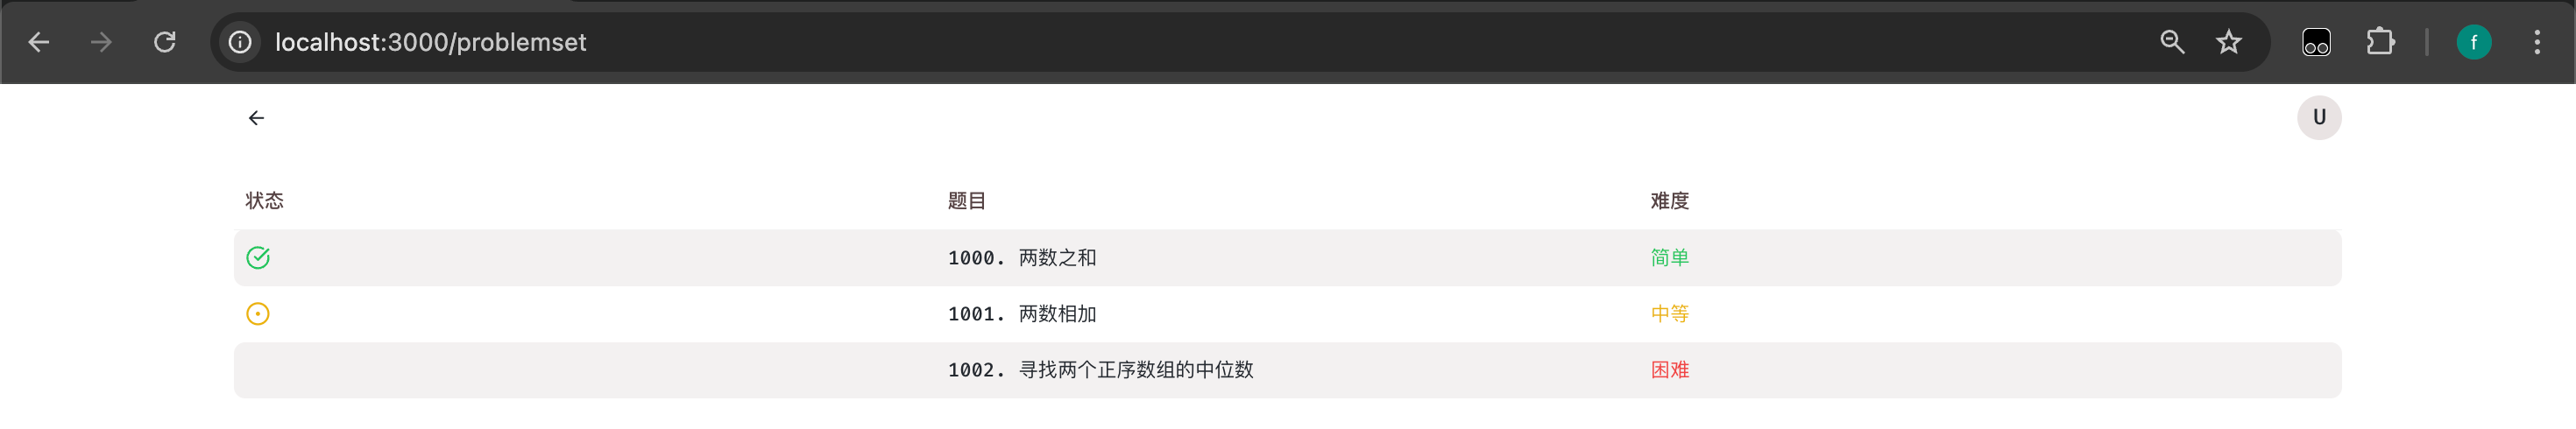
\includegraphics[width=0.78\textwidth]{images/fig6-2.png}
  \caption{题目列表页面截图}
  \label{fig:ch6-problemlist}
\end{figure}

当前工程实现与构建结果表明，系统主线功能已经基本齐备。用户注册登录、题目访问、模板加载、代码提交、结果查看和 AI 反馈展示等操作均可正常完成。与此同时，项目也通过了 \texttt{bun run lint} 与 \texttt{bun run build}，说明当前代码版本在静态检查和生产构建层面不存在明显阻塞问题。综合上述功能用例与构建结果，系统核心流程已具备稳定演示能力。

\section{判题正确性验证}

判题正确性测试是本系统测试中的核心部分，重点在于确认系统能否准确识别不同提交结果类型。本文围绕代表性题目构造了正确程序、编译错误程序、答案错误程序、运行错误程序以及时间超限程序等样例，并对系统返回状态进行逐项核对。对于输出比对相关逻辑，本文同时确认裁剪配置不会破坏结果判定的一致性。

在此处，关键并非题目数量，而是核心状态能否均被准确识别。基于此，本文运用状态覆盖优先的测试方式：围绕一个输入输出比较清晰的代表性题目，分别建立 \texttt{AC}、\texttt{CE}、\texttt{WA}、\texttt{RE}、\texttt{TLE} 等样例，并且逐一核对系统返回的结果。如此一来，更易于说明系统是否具备基本可靠的判题能力。

\begingroup
\small
\setlength{\LTleft}{\fill}
\setlength{\LTright}{\fill}
\setlength{\tabcolsep}{2pt}
\begin{xltabular}{\textwidth}{
P{0.07\textwidth}
P{0.10\textwidth}
>{\hsize=1.20\hsize\RaggedRight\arraybackslash}X
P{0.10\textwidth}
P{0.11\textwidth}
P{0.09\textwidth}
>{\hsize=1.10\hsize\RaggedRight\arraybackslash}X
}
\caption{判题正确性测试结果}\label{tab:ch6-judge-correctness}\\
\toprule
编号 & 测试类型 & 输入代码特征 & 预期状态 & 实际状态 & 是否通过 & 备注 \\
\midrule
\endfirsthead
\multicolumn{7}{c}{续表\thetable}\\
\toprule
编号 & 测试类型 & 输入代码特征 & 预期状态 & 实际状态 & 是否通过 & 备注 \\
\midrule
\endhead
\bottomrule
\endfoot
J-01 & 正确程序 & 全用例可过 & AC & AC & 通过 & 图~\ref{fig:ch5-submit} \\
J-02 & 编译错误程序 & 缺分号等 & CE & CE & 通过 & 图~\ref{fig:ch5-submission-list} \\
J-03 & 答案错误程序 & 输出与标答不符 & WA & WA & 通过 & 图~\ref{fig:ch5-submission-list} \\
J-04 & 运行错误程序 & 运行期异常退出 & RE & RE & 通过 & \texttt{abort()}；图~\ref{fig:ch5-submission-list} \\
J-05 & 时间超限程序 & 死循环/长期无响应 & TLE & TLE & 通过 & 图~\ref{fig:ch5-submission-list} \\
\bottomrule
\end{xltabular}
\endgroup

\begingroup
\small
\setlength{\LTleft}{\fill}
\setlength{\LTright}{\fill}
\setlength{\tabcolsep}{2pt}
\begin{xltabular}{\textwidth}{
P{0.07\textwidth}
P{0.11\textwidth}
>{\hsize=1.00\hsize\RaggedRight\arraybackslash}X
>{\hsize=1.10\hsize\RaggedRight\arraybackslash}X
>{\hsize=1.20\hsize\RaggedRight\arraybackslash}X
}
\caption{不同错误类型样例与系统返回状态}\label{tab:ch6-error-samples}\\
\toprule
编号 & 错误类型 & 构造方式 & 页面表现 & 结果说明 \\
\midrule
\endfirsthead
\multicolumn{5}{c}{续表\thetable}\\
\toprule
编号 & 错误类型 & 构造方式 & 页面表现 & 结果说明 \\
\midrule
\endhead
\bottomrule
\endfoot
E-01 & 编译错误 & 删分号/未声明变量等 & 返回 CE 并展示编译信息 & 语法层失败可识别 \\
E-02 & 答案错误 & 固定错答或漏分支 & 返回 WA 并保留用例信息 & 标答比对可用 \\
E-03 & 运行错误 & \texttt{abort()} 等 & 返回 RE & 运行期异常可识别 \\
E-04 & 时间超限 & \texttt{while(1)\{\}} & 返回 TLE & 时限控制可用 \\
\bottomrule
\end{xltabular}
\endgroup

判题正确性是本系统最核心的验证内容，实际测试表明，系统在接收到提交后，能够依次完成前置校验、编译、运行和结果判定，并对 \texttt{AC}、\texttt{CE}、\texttt{WA}、\texttt{RE} 和 \texttt{TLE} 等核心状态给出与预期一致的返回结果。这说明系统已具备基本可靠的判题能力。针对容器清理、远程 Docker 连接与输出记录等边界条件，本文在异常路径中给出状态回写与日志追踪策略\cite{alemu2023serverless,kubernetesdocs}。

\section{安全隔离与恶意代码防护验证}

除常规判题状态验证之外，本文还补充了高风险样例来检验隔离边界。测试重点覆盖三类行为：进程滥用、内存滥用、网络外联。并且这些样例全部走与普通提交一致的默认判题链路，不额外增加特权配置，这样才能更真实地验证沙箱默认策略是否足够有效。

\begingroup
\small
\setlength{\LTleft}{\fill}
\setlength{\LTright}{\fill}
\setlength{\tabcolsep}{2pt}
\begin{xltabular}{\textwidth}{
P{0.08\textwidth}
P{0.16\textwidth}
>{\hsize=1.00\hsize\RaggedRight\arraybackslash}X
P{0.14\textwidth}
>{\hsize=1.30\hsize\RaggedRight\arraybackslash}X
}
\caption{恶意代码防护验证结果}\label{tab:ch6-security-cases}\\
\toprule
编号 & 攻击场景 & 样例行为 & 实际状态 & 验证结论 \\
\midrule
\endfirsthead
\multicolumn{5}{c}{续表\thetable}\\
\toprule
编号 & 攻击场景 & 样例行为 & 实际状态 & 验证结论 \\
\midrule
\endhead
\bottomrule
\endfoot
S-01 & 进程滥用 & 循环 \texttt{fork()} & TLE/RE & 容器内终止，未拖垮宿主 \\
S-02 & 内存滥用 & 超大连续申请 & MLE & 内存上限生效 \\
S-03 & 网络外联 & 容器内连公网 & RE & 默认网络隔离生效 \\
\bottomrule
\end{xltabular}
\endgroup

上述结果表明，平台当前的判题沙箱不仅能够处理普通错误类型，也能对高风险样例形成有效约束。对应样例代码见附录中的恶意代码样例，便于复核与复现实验。

\begin{figure}[htbp]
  \centering
  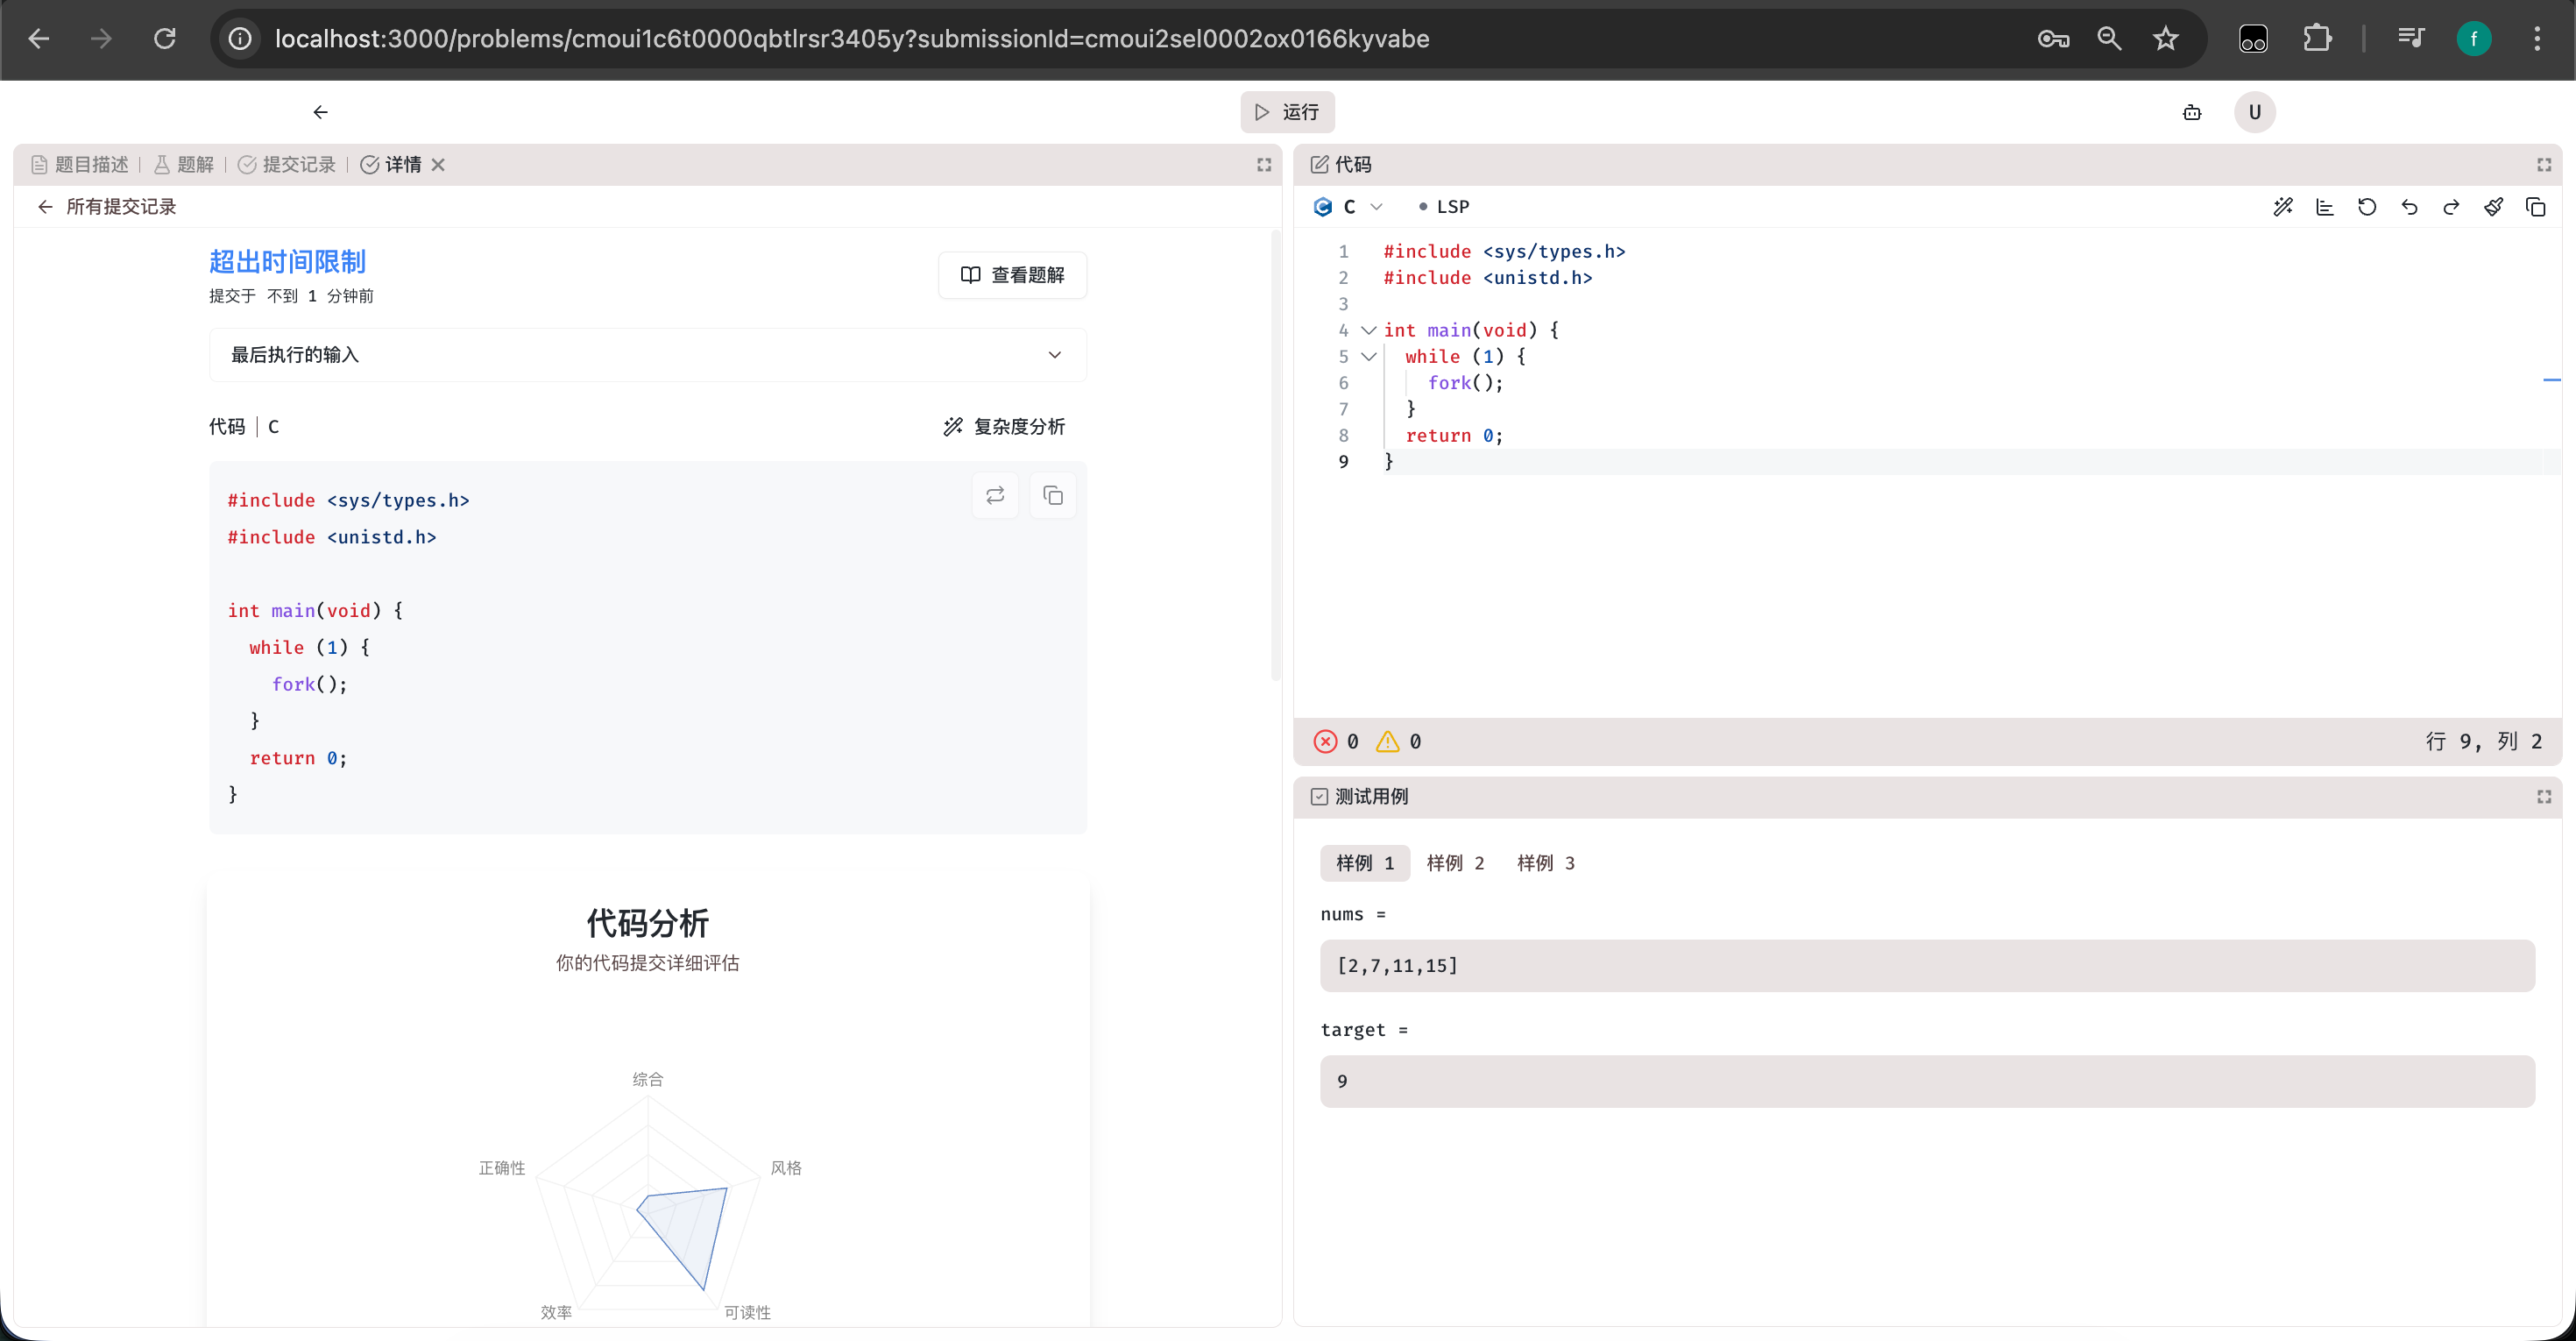
\includegraphics[width=0.92\textwidth]{images/fig6-10.png}
  \caption{进程滥用样例提交结果截图}
  \label{fig:ch6-security-fork}
\end{figure}

\begin{figure}[htbp]
  \centering
  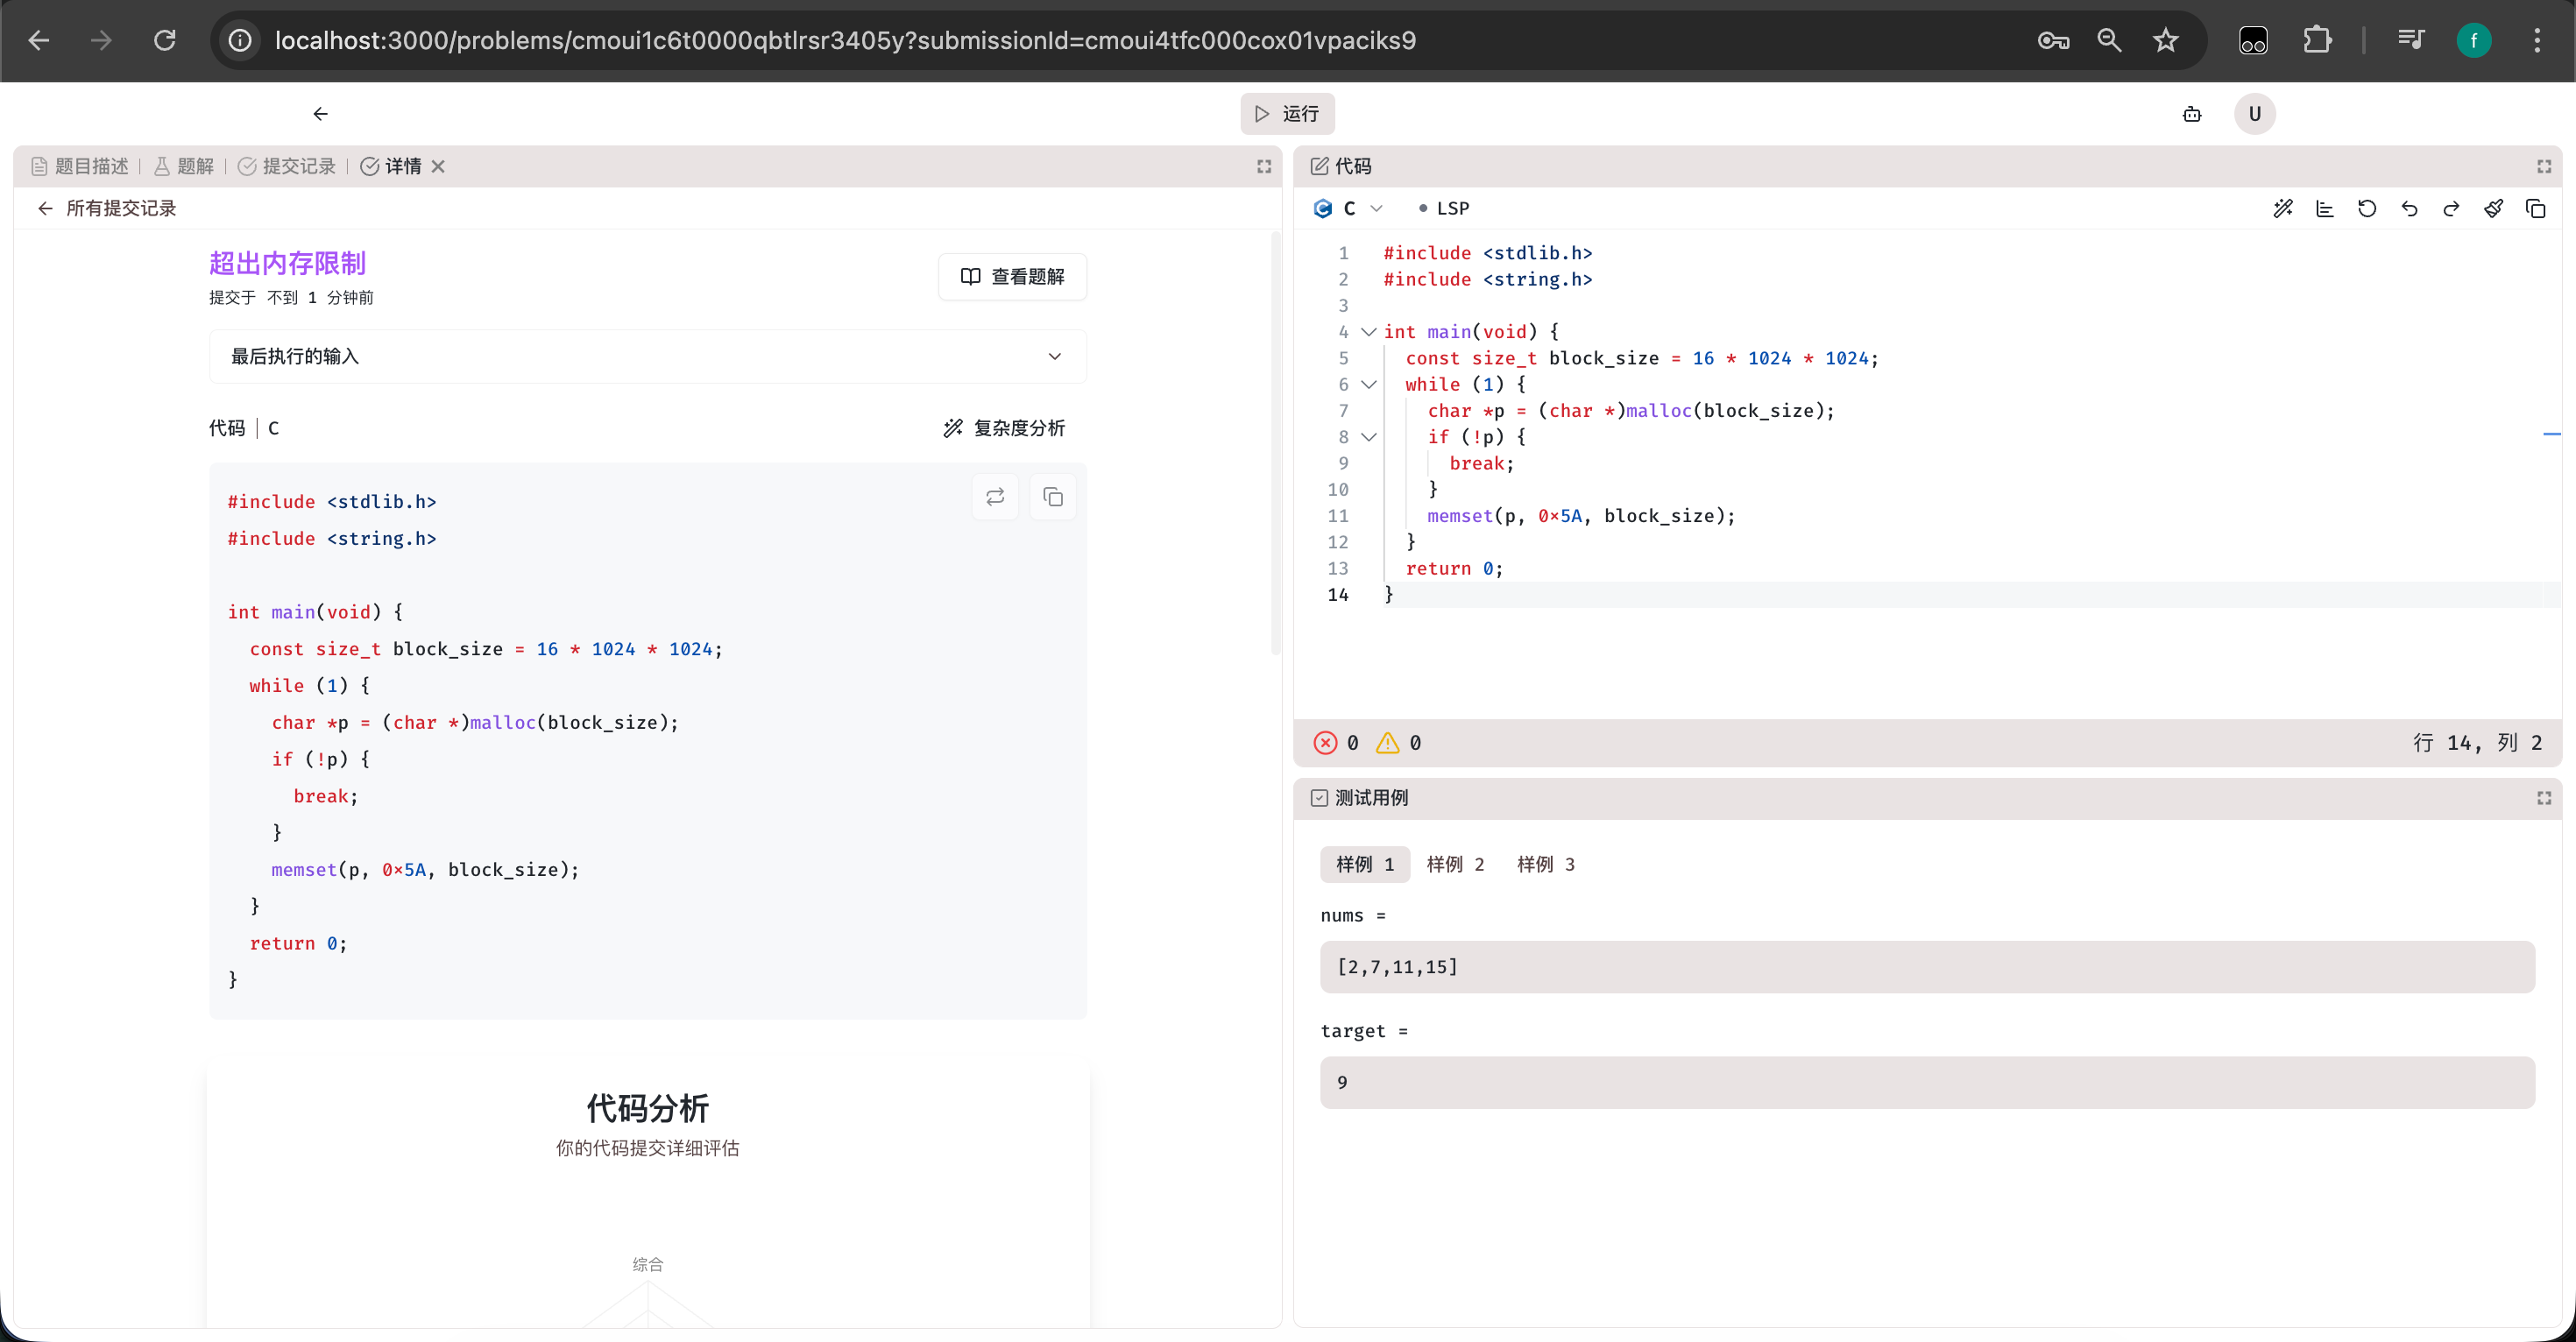
\includegraphics[width=0.92\textwidth]{images/fig6-11.png}
  \caption{内存滥用样例提交结果截图}
  \label{fig:ch6-security-memory}
\end{figure}

\begin{figure}[htbp]
  \centering
  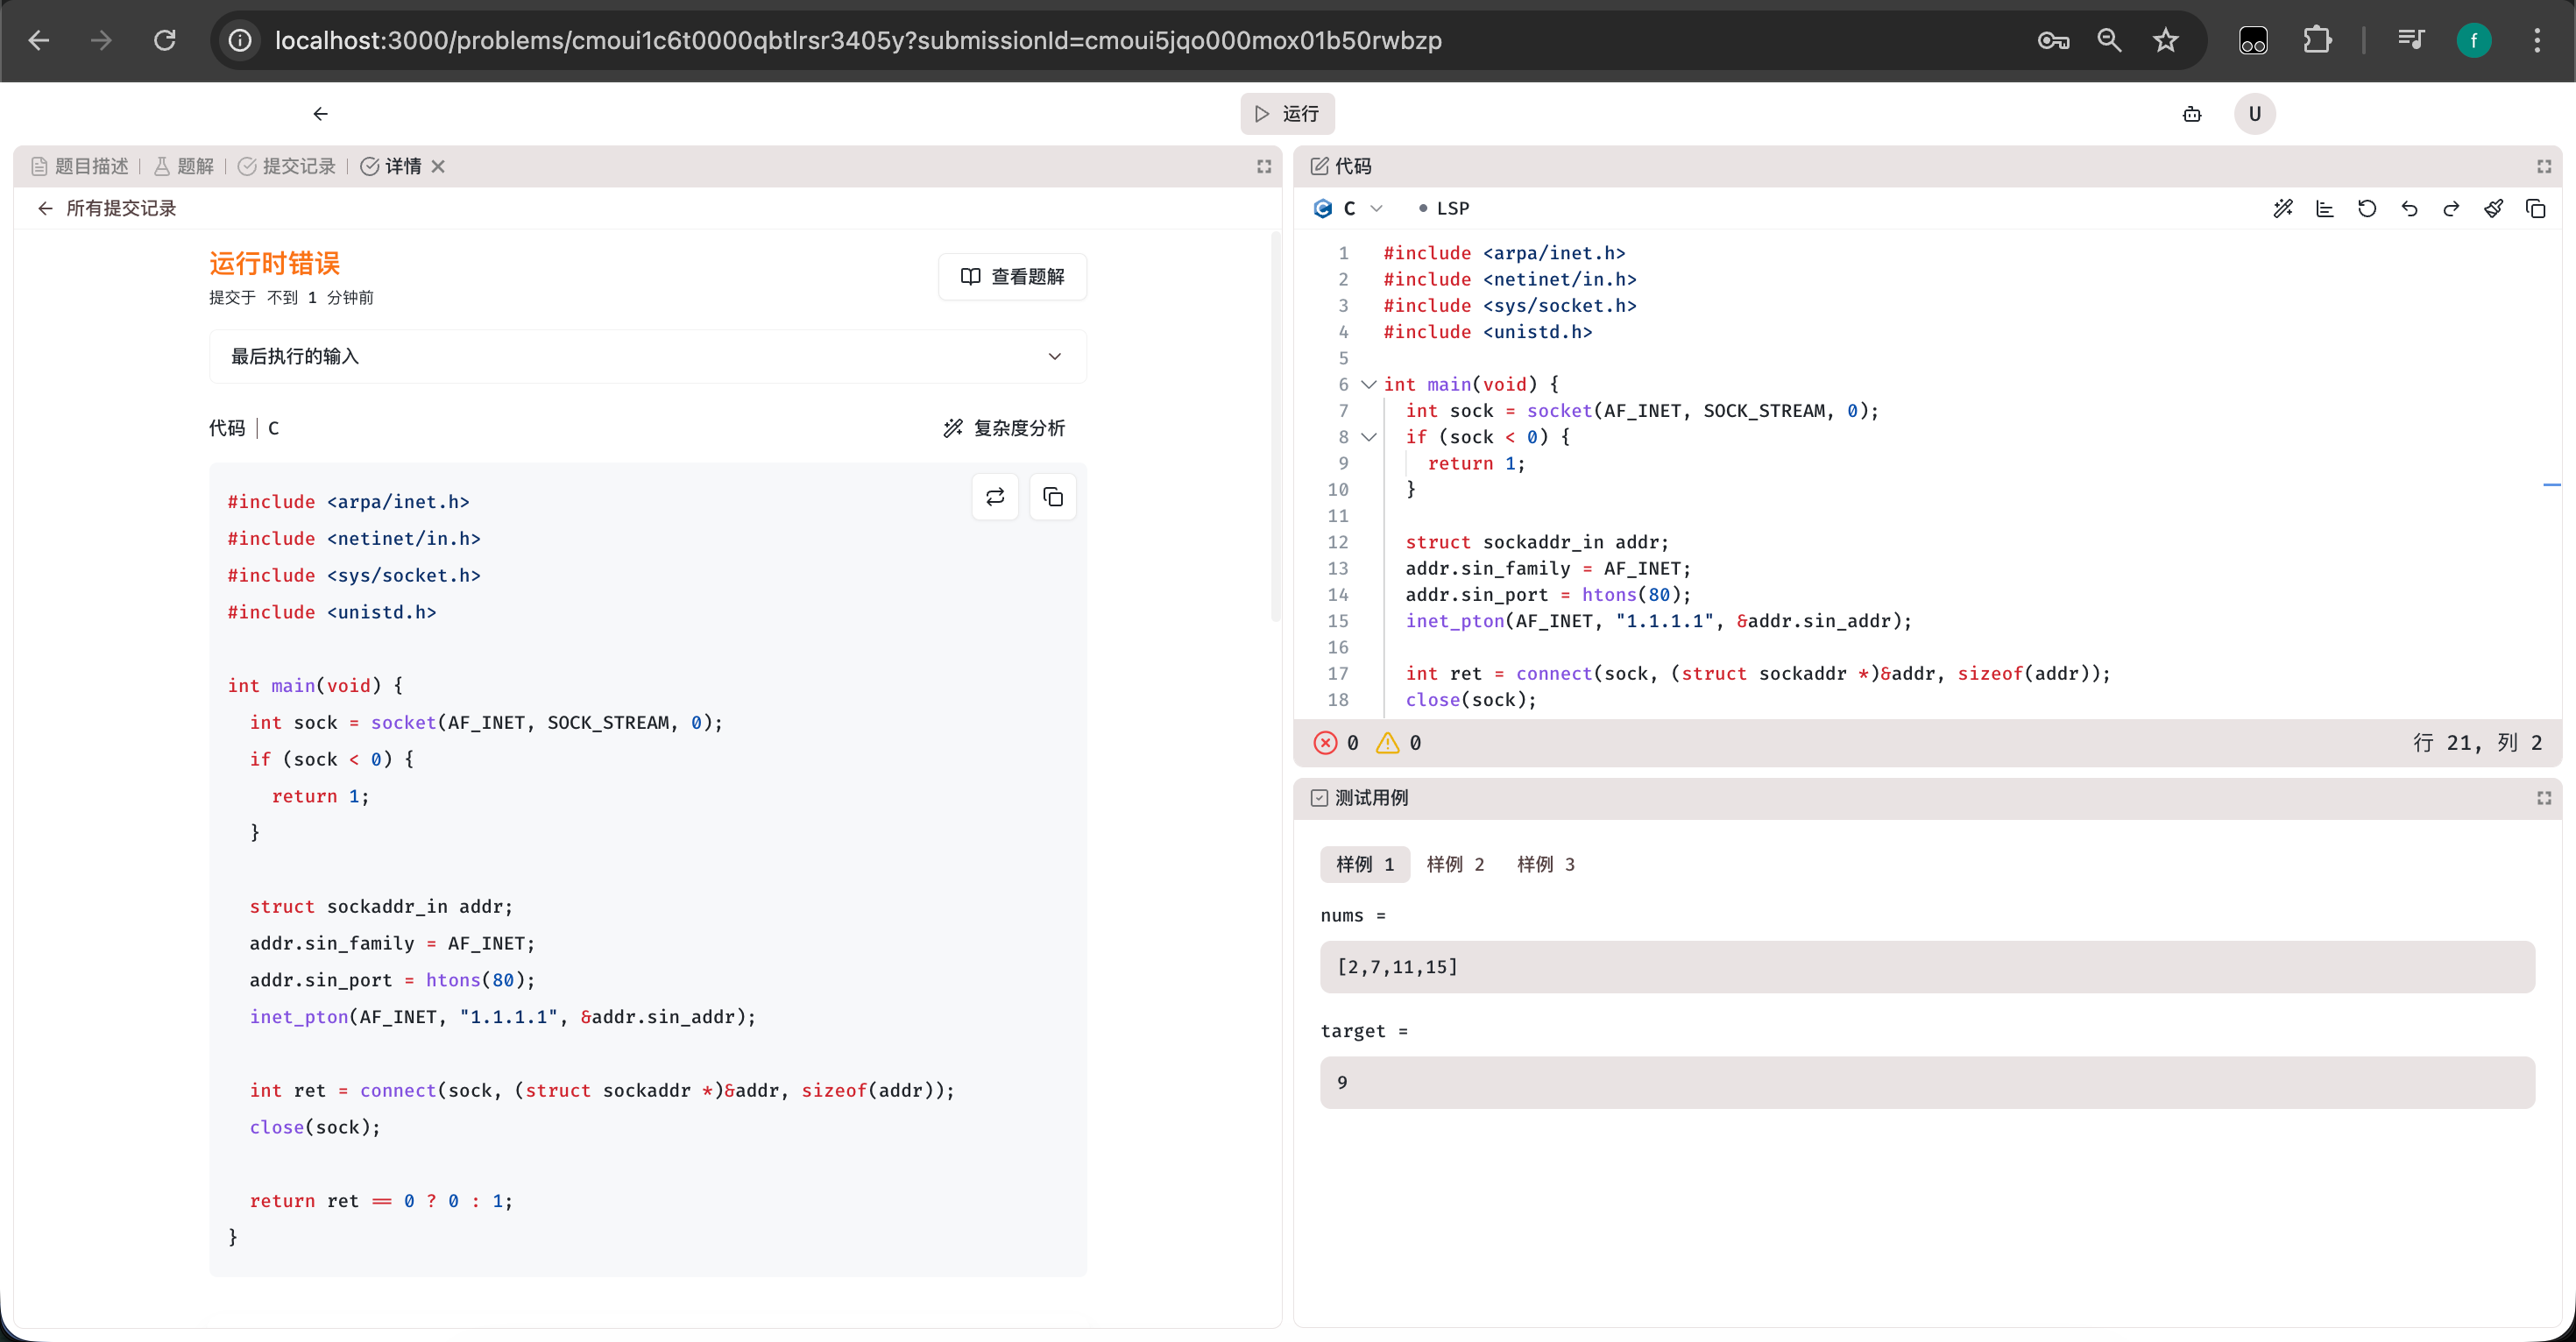
\includegraphics[width=0.92\textwidth]{images/fig6-12.png}
  \caption{网络外联样例提交结果截图}
  \label{fig:ch6-security-network}
\end{figure}

图~\ref{fig:ch6-security-fork}、图~\ref{fig:ch6-security-memory} 与图~\ref{fig:ch6-security-network} 分别对应进程滥用、内存滥用和网络外联三类场景。页面结果与表~\ref{tab:ch6-security-cases} 中的状态记录一致，能够直接展示平台在默认判题链路下对恶意行为的约束效果。

\section{AI 辅助反馈效果验证}

AI 辅助反馈效果分析选择了若干具有代表性的提交样例，例如编译错误、逻辑错误、低效实现和风格较差的代码，用于观察系统输出的复杂度估计、评分结果和反馈内容是否具有合理性。该部分测试的关注重点不是 AI 是否绝对正确，而是其输出是否与客观判题结果一致、是否具有解释价值、是否避免直接给出完整答案以及是否能够帮助学生理解问题。

\begingroup
\small
\setlength{\LTleft}{\fill}
\setlength{\LTright}{\fill}
\setlength{\tabcolsep}{2pt}
\begin{xltabular}{\textwidth}{
P{0.07\textwidth}
P{0.13\textwidth}
>{\hsize=1.00\hsize\RaggedRight\arraybackslash}X
>{\hsize=1.10\hsize\RaggedRight\arraybackslash}X
>{\hsize=1.00\hsize\RaggedRight\arraybackslash}X
>{\hsize=0.90\hsize\RaggedRight\arraybackslash}X
}
\caption{AI 辅助反馈效果示例}\label{tab:ch6-ai-feedback-cases}\\
\toprule
编号 & 提交场景 & AI 输出重点 & 预期评价维度 & 实际情况 & 展示价值 \\
\midrule
\endfirsthead
\multicolumn{6}{c}{续表\thetable}\\
\toprule
编号 & 提交场景 & AI 输出重点 & 预期评价维度 & 实际情况 & 展示价值 \\
\midrule
\endhead
\bottomrule
\endfoot
A-01 & 编译错误代码 & 原因/位置/修改提示 & 指语法问题、少代写 & 指出缺分号等 & 可用 \\
A-02 & 答案错误代码 & 逻辑/边界提示 & 解释 WA 主因 & 指出恒返 \texttt{[0,0]} & 可用；图~\ref{fig:ch6-ai-wa} \\
A-03 & 低效正确代码 & 复杂度与优化方向 & 复杂度合理 & \(O(N^2)\)/\(O(1)\)，建议哈希 & 可用；图~\ref{fig:ch5-ai-feedback} \\
A-04 & 可读性较差代码 & 命名/结构/风格 & 结构化意见 & 风格约 30、可读约 35 & 可用；图~\ref{fig:ch6-ai-readability} \\
\bottomrule
\end{xltabular}
\endgroup

\begin{figure}[htbp]
  \centering
  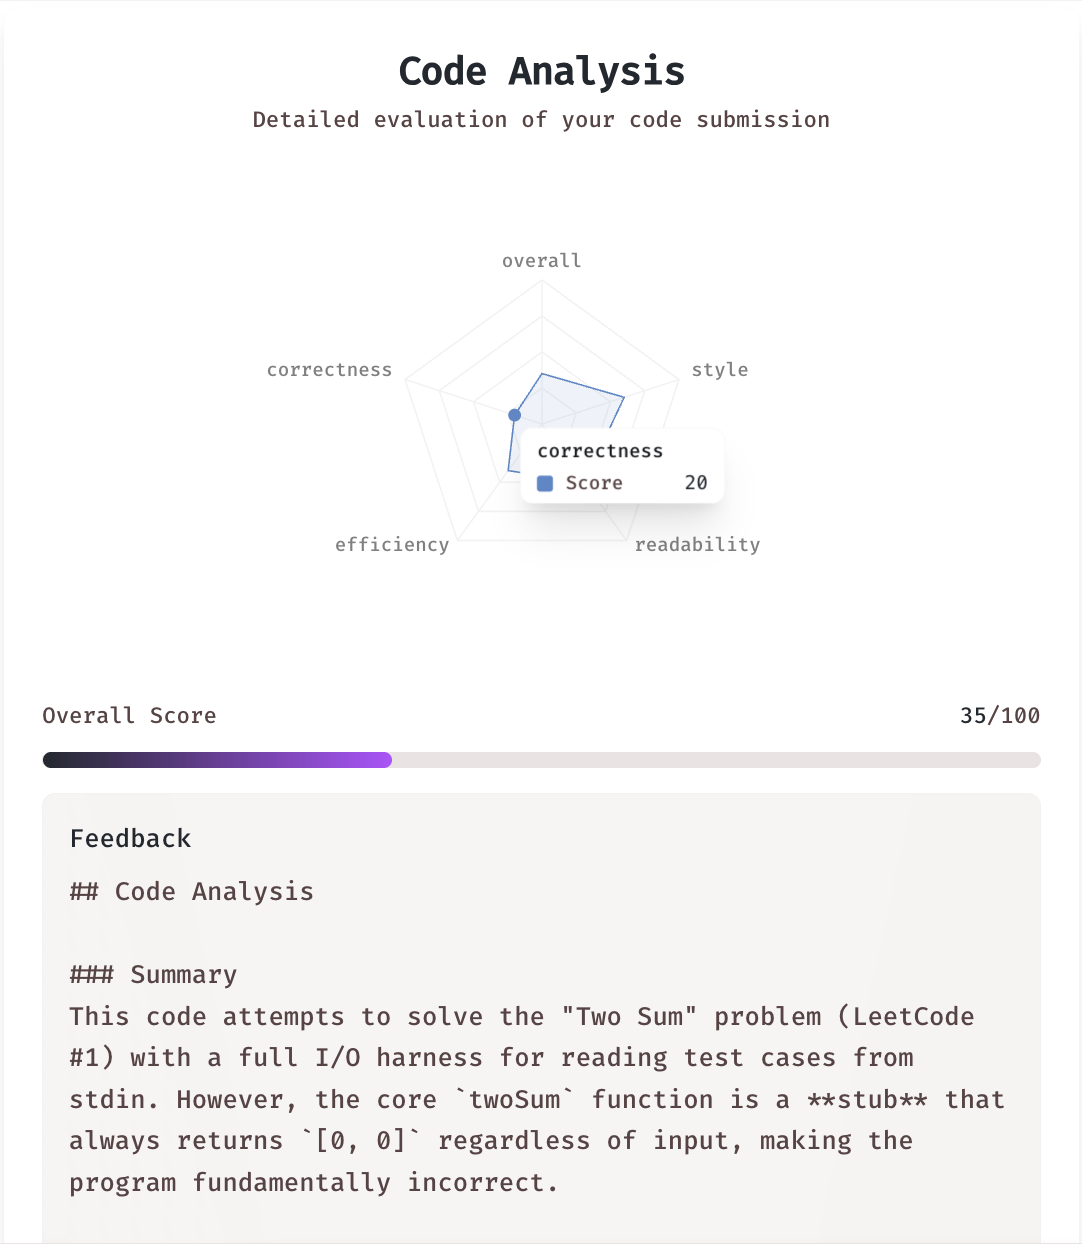
\includegraphics[width=0.72\textwidth]{images/fig6-1.png}
  \caption{答案错误代码的 AI 分析结果截图}
  \label{fig:ch6-ai-wa}
\end{figure}

\begin{figure}[htbp]
  \centering
  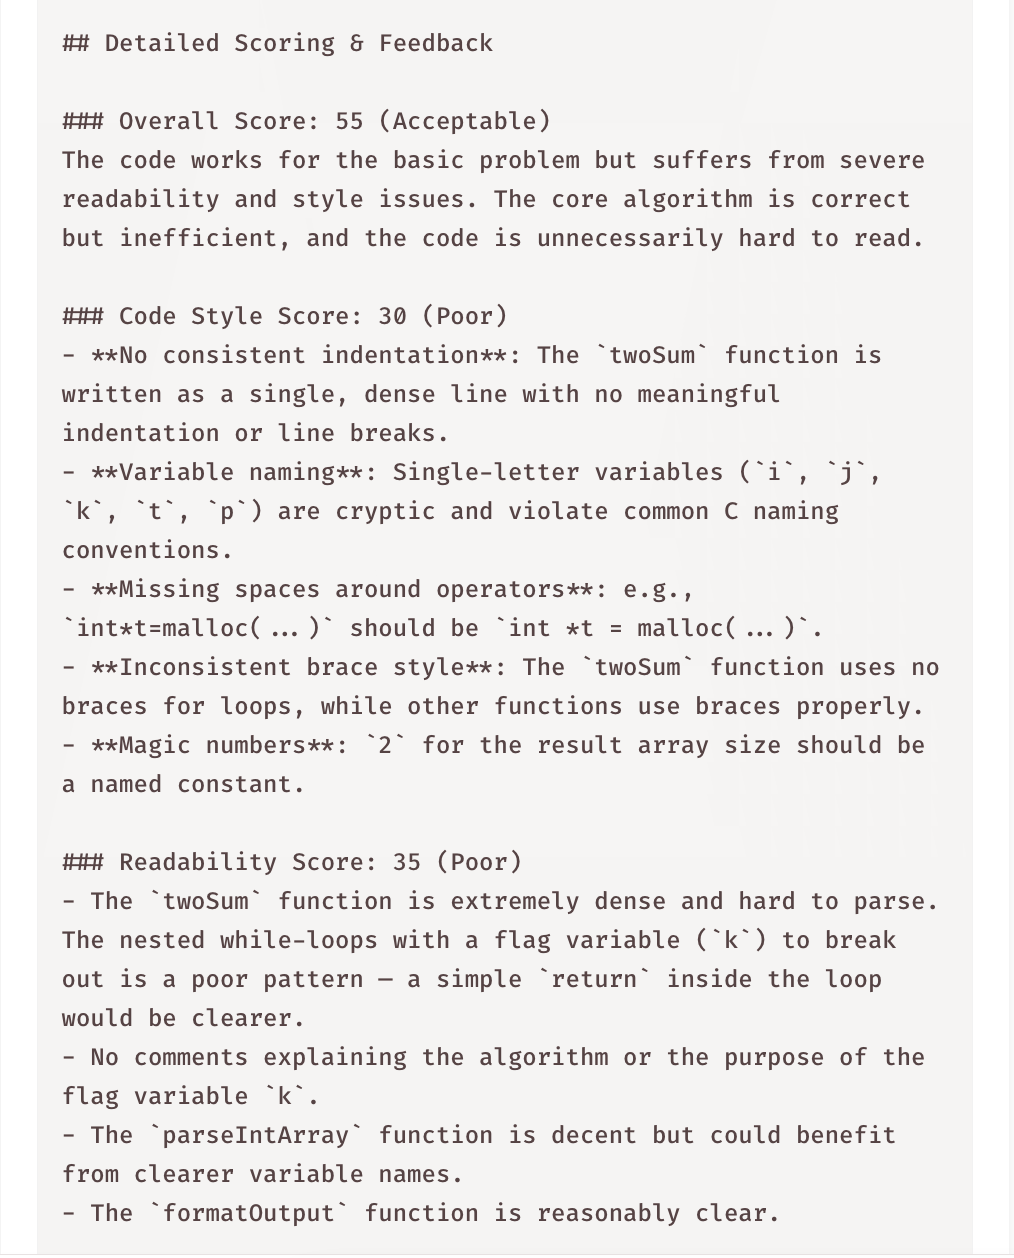
\includegraphics[width=0.72\textwidth]{images/fig6-3.png}
  \caption{可读性较差代码的 AI 分析结果截图}
  \label{fig:ch6-ai-readability}
\end{figure}

AI 辅助反馈部分作为客观判题之后的附加分析存在。从样例结果可见，AI 对编译错误、答案错误、低效正确代码和可读性较差代码都能给出与提交情形基本一致的解释和改进方向，说明该模块已经能够起到一定的学习支持作用，但它并不替代判题结果本身。

\section{工作区交互与多终端适配验证}

\begingroup
\small
\setlength{\LTleft}{\fill}
\setlength{\LTright}{\fill}
\setlength{\tabcolsep}{2pt}
\begin{xltabular}{\textwidth}{
P{0.07\textwidth}
P{0.16\textwidth}
P{0.12\textwidth}
>{\hsize=1.20\hsize\RaggedRight\arraybackslash}X
>{\hsize=0.90\hsize\RaggedRight\arraybackslash}X
}
\caption{界面与交互能力测试结果}\label{tab:ch6-interaction}\\
\toprule
编号 & 测试项 & 实际结果 & 结果说明 & 截图对应 \\
\midrule
\endfirsthead
\multicolumn{5}{c}{续表\thetable}\\
\toprule
编号 & 测试项 & 实际结果 & 结果说明 & 截图对应 \\
\midrule
\endhead
\bottomrule
\endfoot
I-01 & 响应式布局 & 通过 & 窄屏主流程可读 & 图~\ref{fig:mobile-workspace} \\
I-02 & 多语言切换 & 通过 & 界面与题面语种一致 & 图~\ref{fig:lang-switch} \\
I-03 & 深浅色主题 & 通过 & 页/工作区/代码区配色一致 & 图~\ref{fig:dark-theme-workspace} \\
I-04 & 编辑器 AI 工具栏 & 通过 & Diff 可看改动，未静默覆盖 & 图~\ref{fig:diff-view} \\
I-05 & 机器人问答面板 & 通过 & 回答绑定当前代码上下文 & 图~\ref{fig:ai-chat-panel} \\
I-06 & 语言服务 LSP 体验 & 通过 & 连接态可见；错误可出诊断 & 图~\ref{fig:ch6-lsp} \\
\bottomrule
\end{xltabular}
\endgroup

\begin{figure}[htbp]
  \centering
  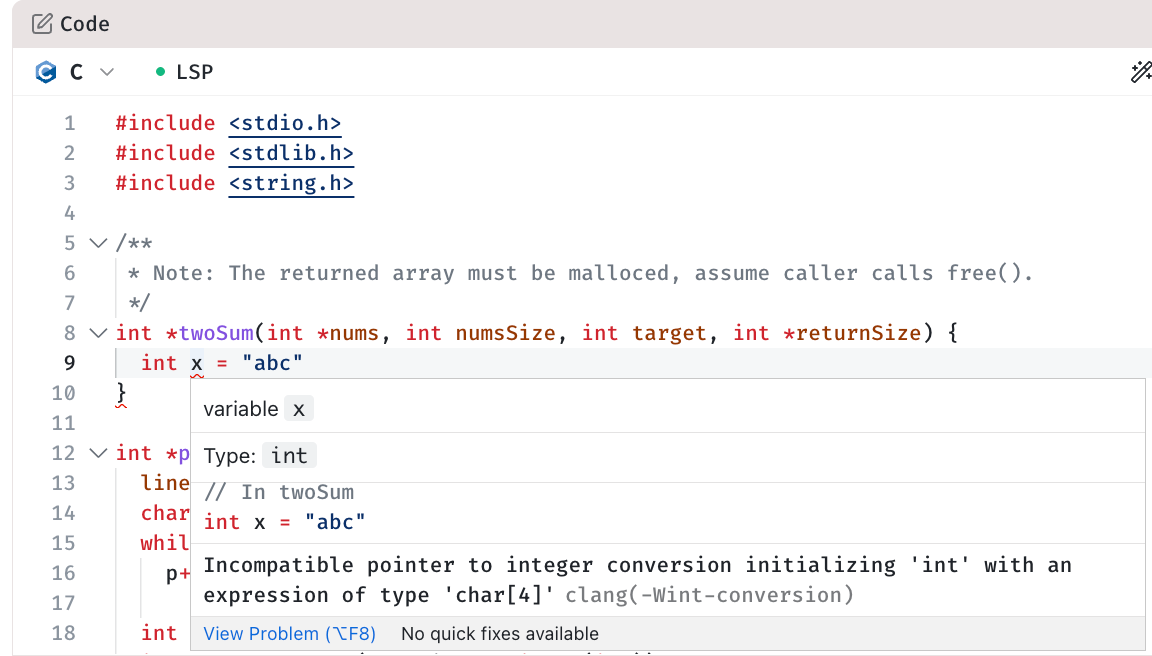
\includegraphics[width=0.92\linewidth]{images/fig6-9.png}
  \caption{LSP 连接指示与编辑器诊断标记同屏截图}
  \label{fig:ch6-lsp}
\end{figure}

\begin{figure}[htbp]
  \centering
  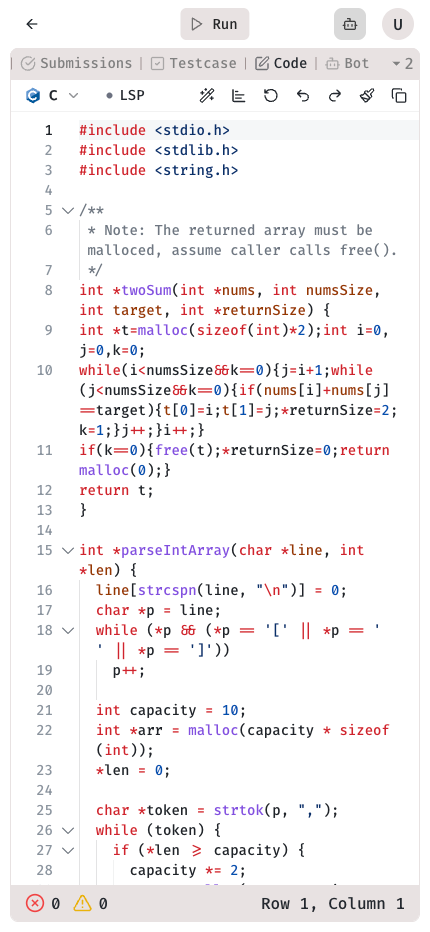
\includegraphics[width=0.30\textwidth]{images/fig6-4.png}
  \caption{移动端题目工作区截图}
  \label{fig:mobile-workspace}
\end{figure}

\begin{figure}[htbp]
  \centering
  \begin{subfigure}{0.49\textwidth}
    \centering
    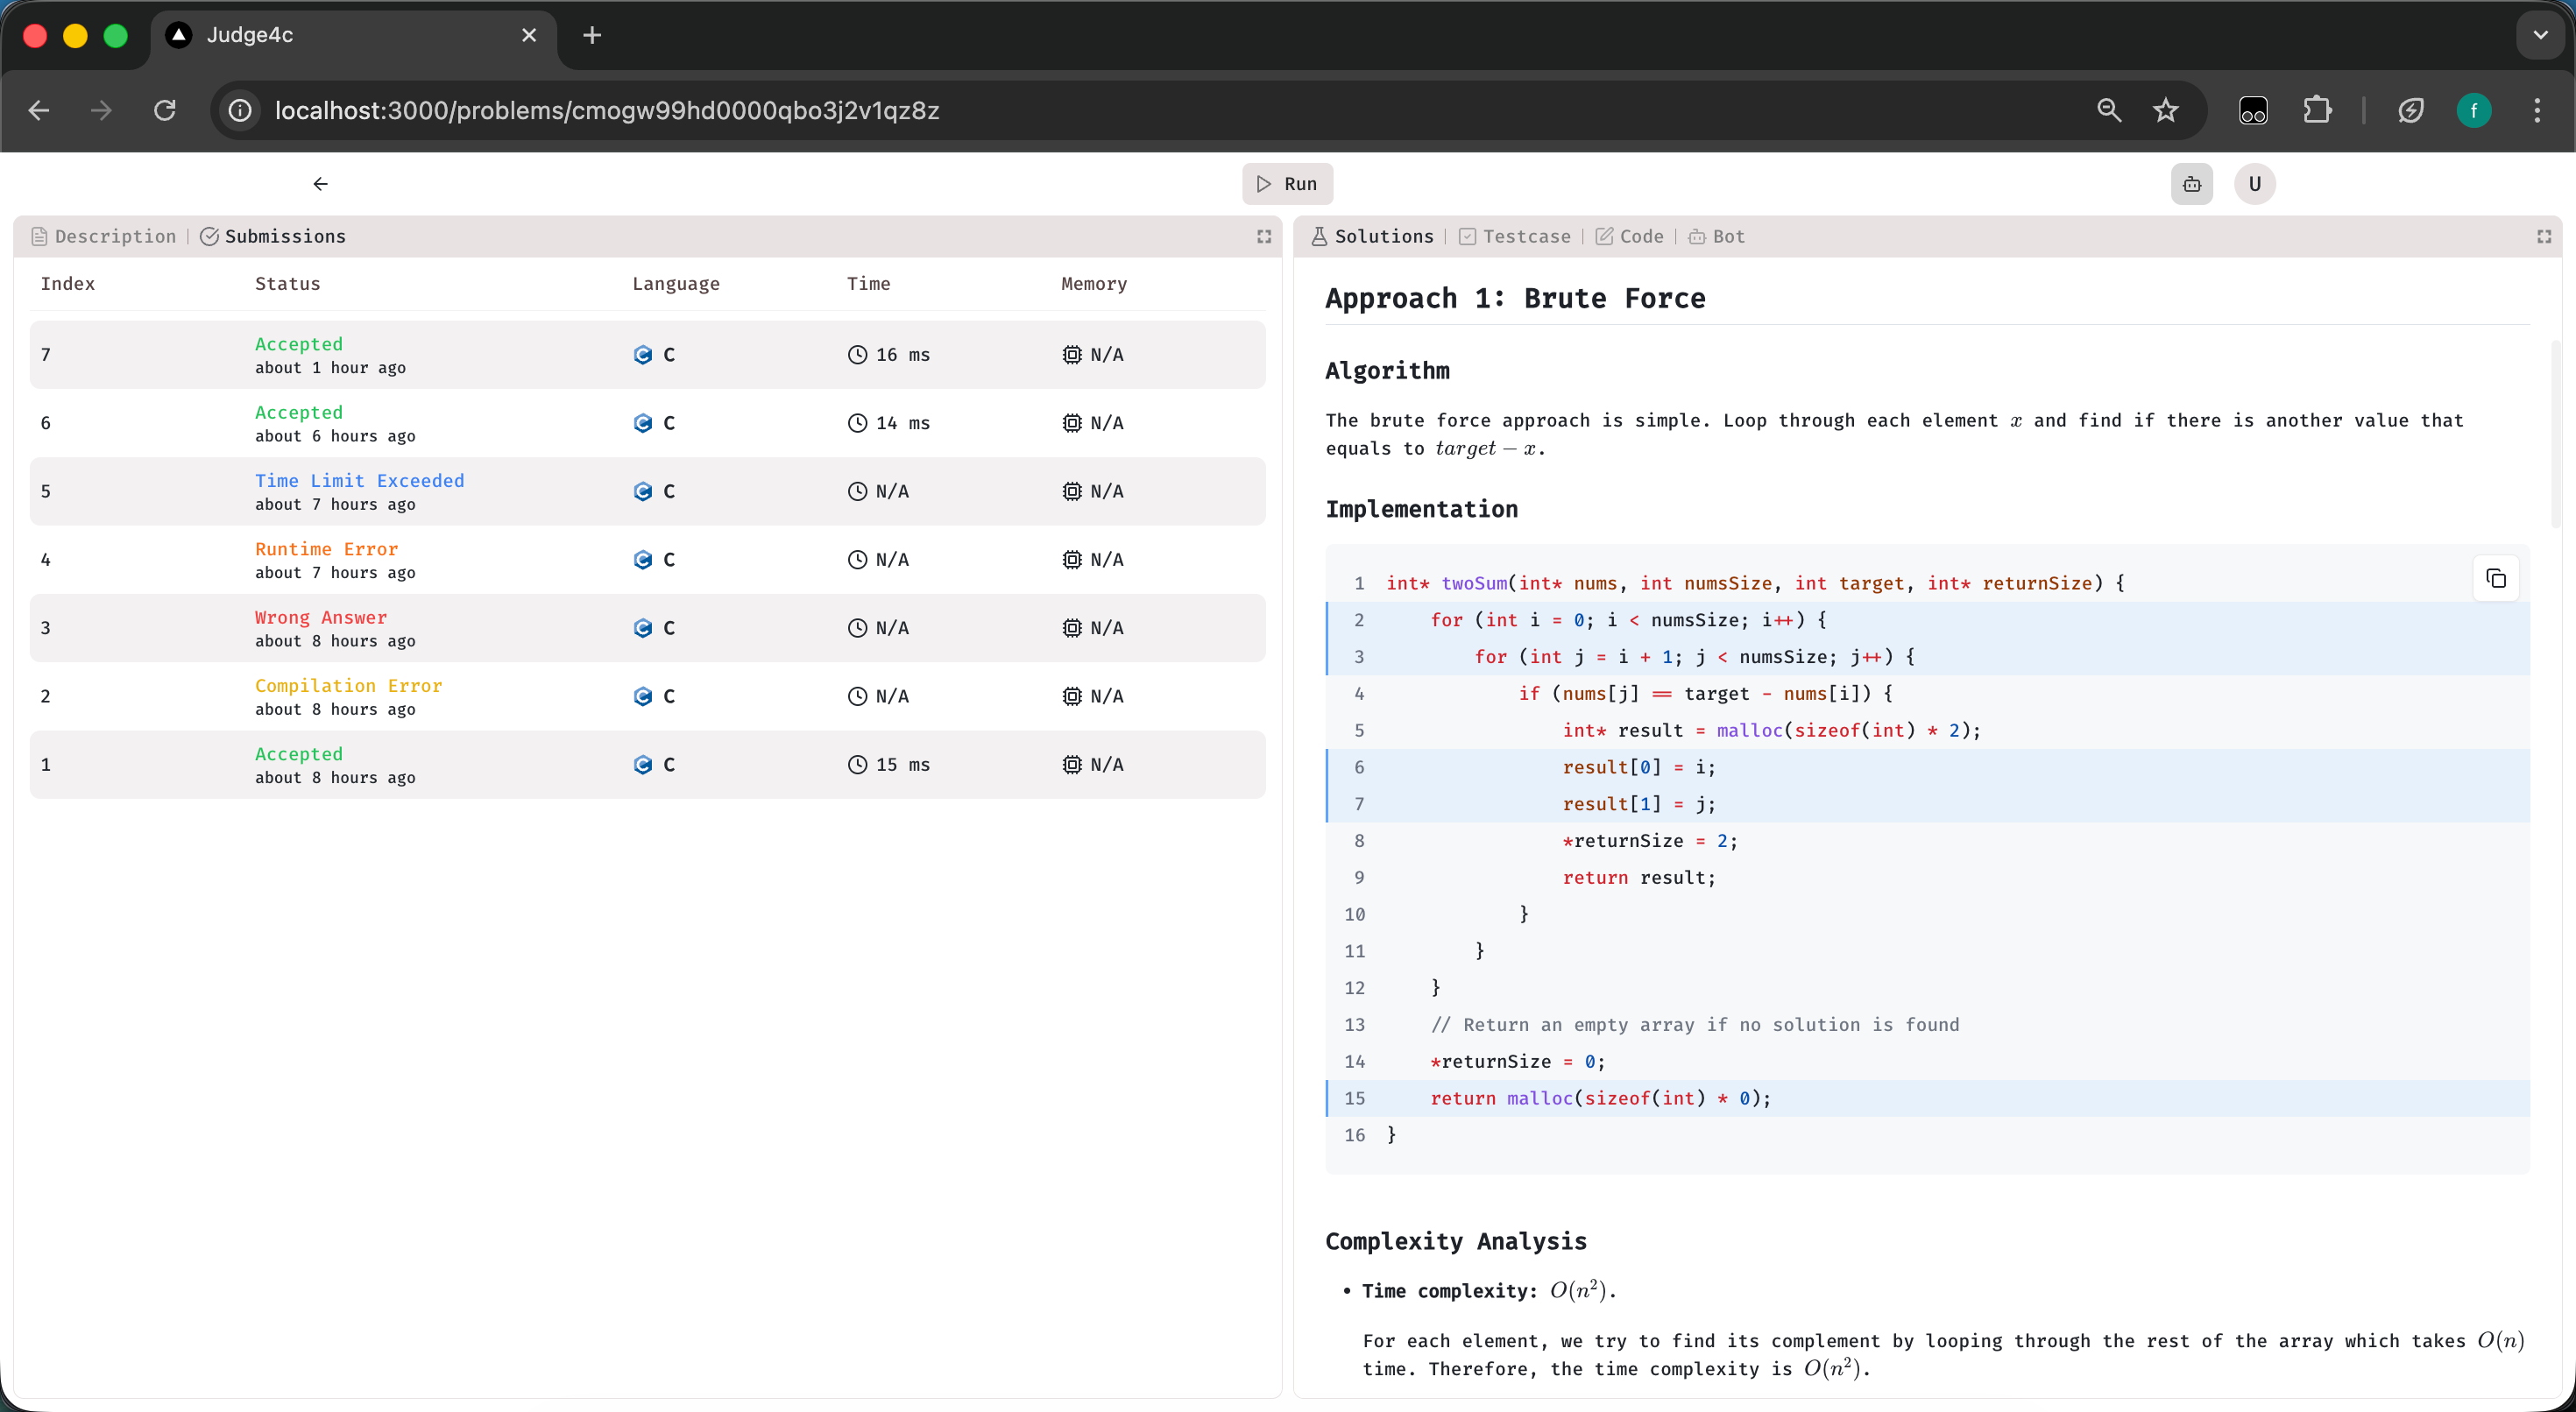
\includegraphics[width=\textwidth]{images/fig6-5a.png}
    \caption{英文界面与题面内容}
  \end{subfigure}
  \hfill
  \begin{subfigure}{0.49\textwidth}
    \centering
    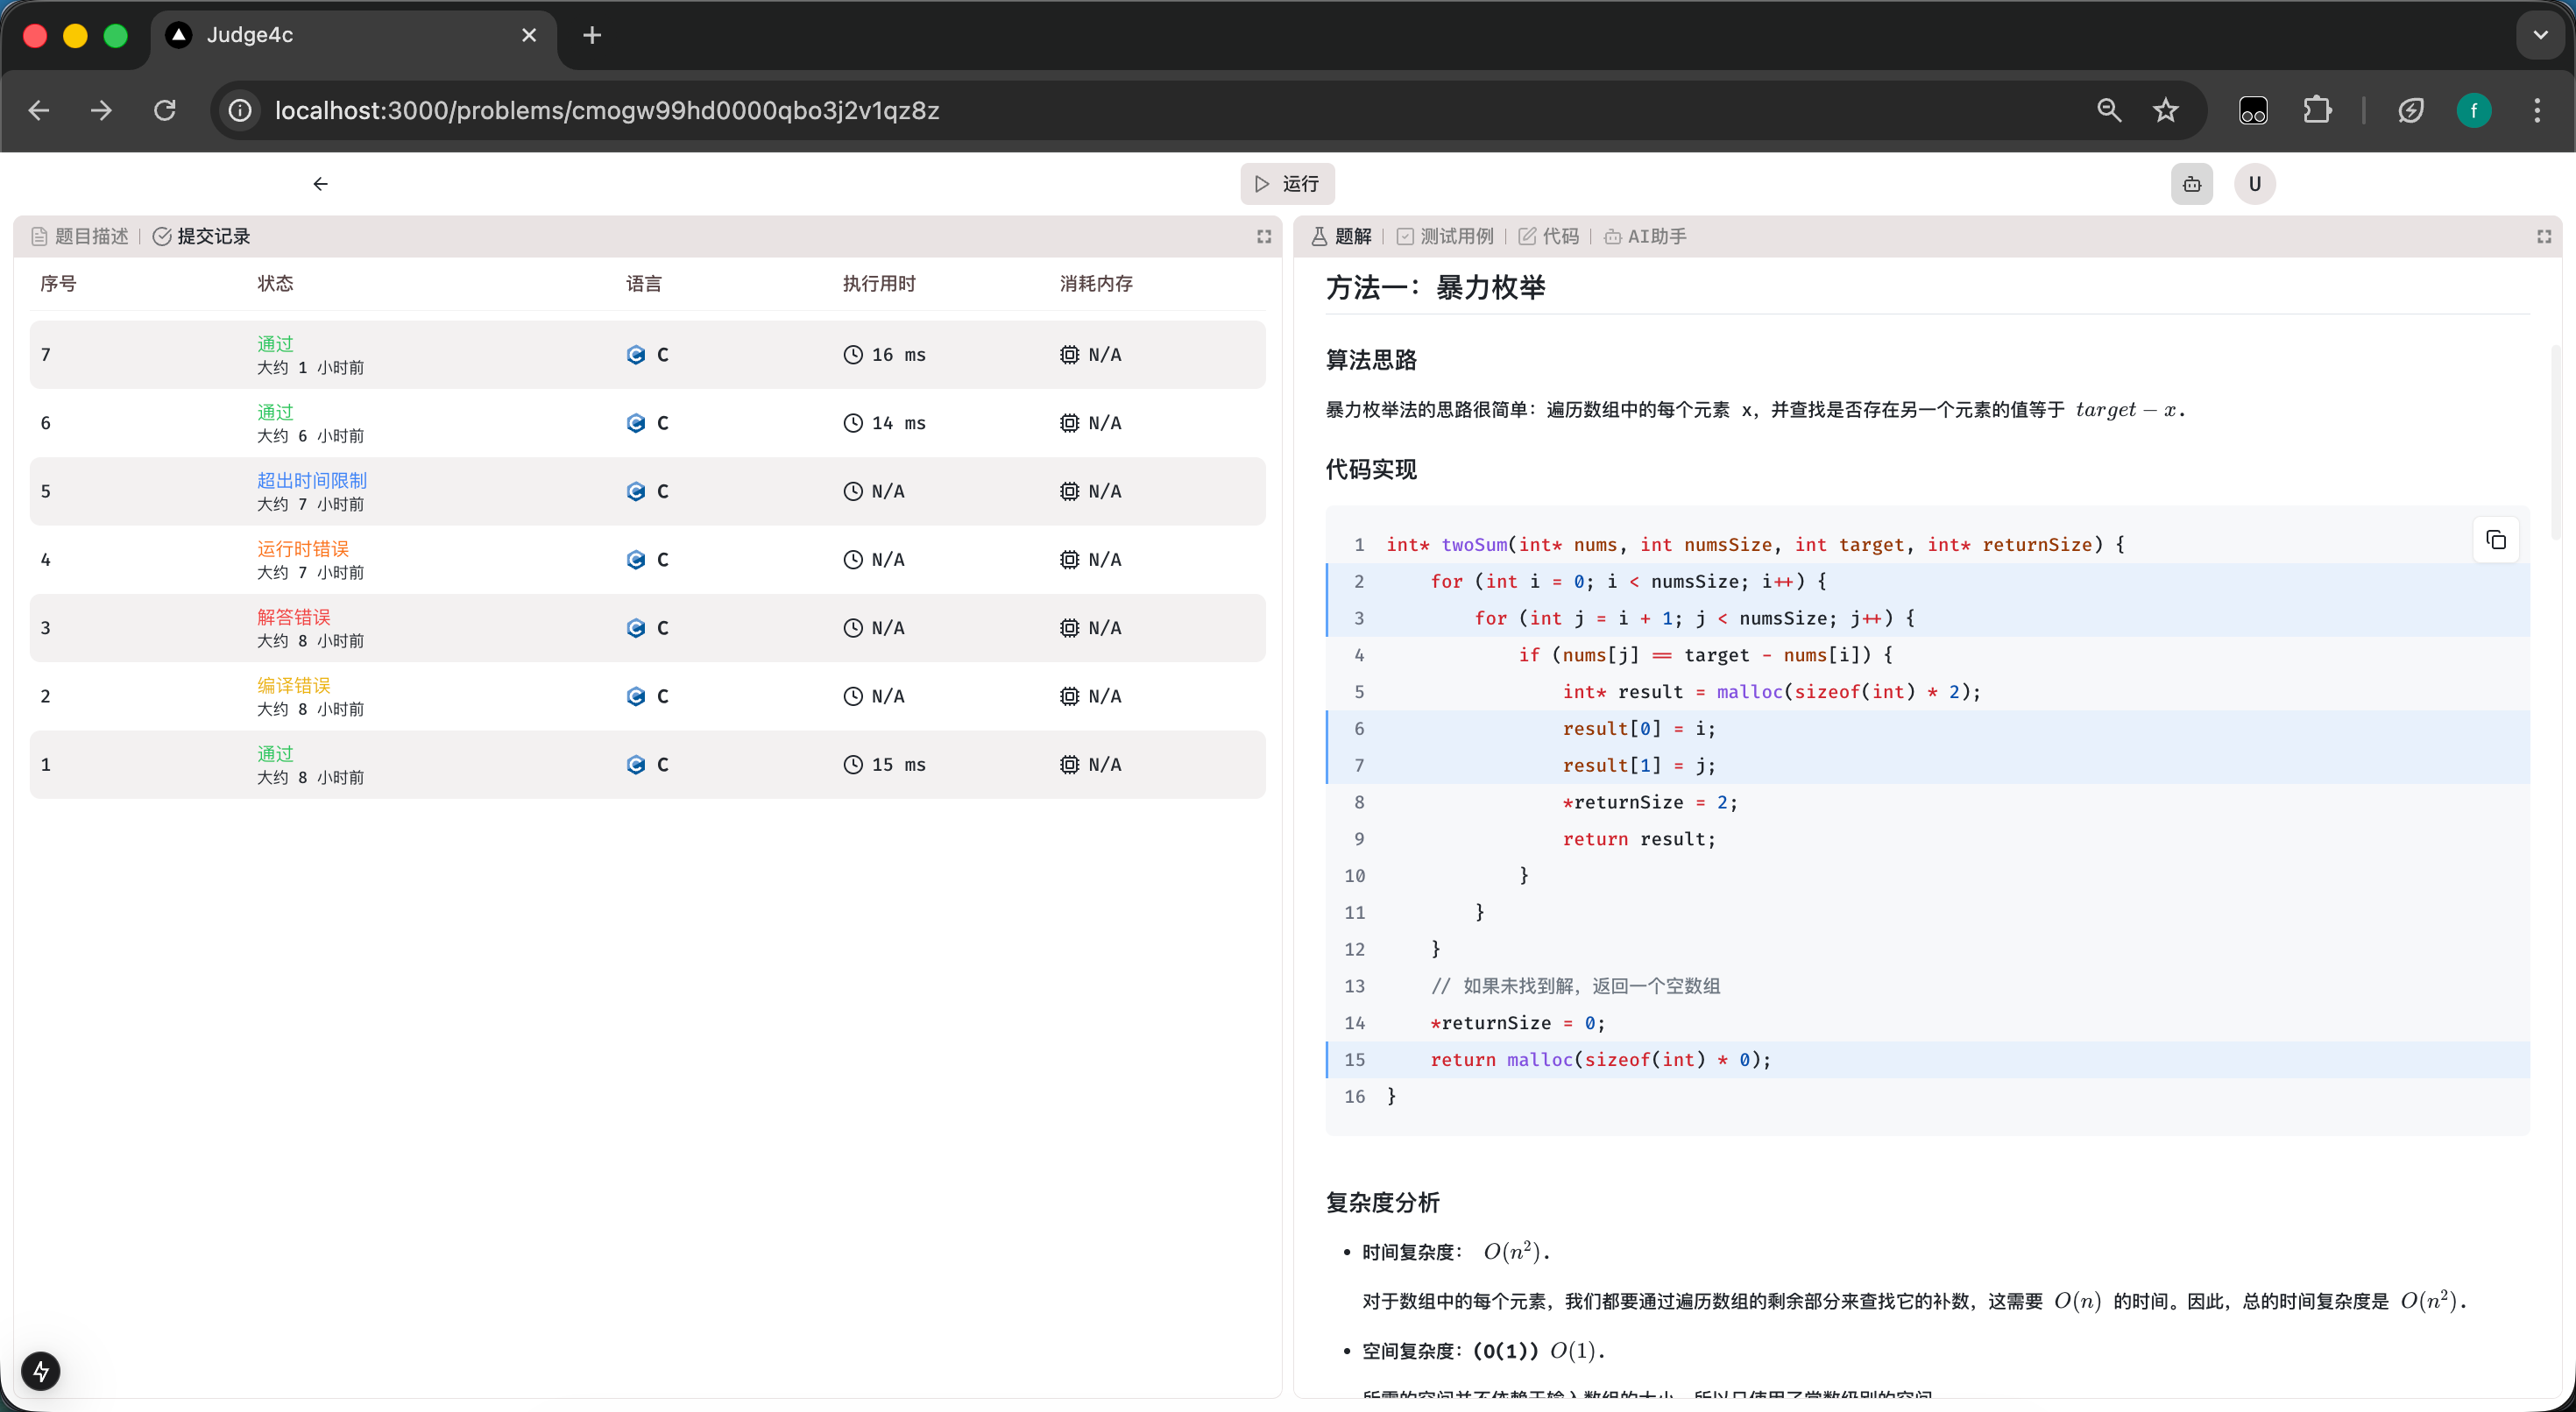
\includegraphics[width=\textwidth]{images/fig6-5b.png}
    \caption{中文界面与题面内容}
  \end{subfigure}
  \caption{中英文界面切换效果截图}
  \label{fig:lang-switch}
\end{figure}

\begin{figure}[htbp]
  \centering
  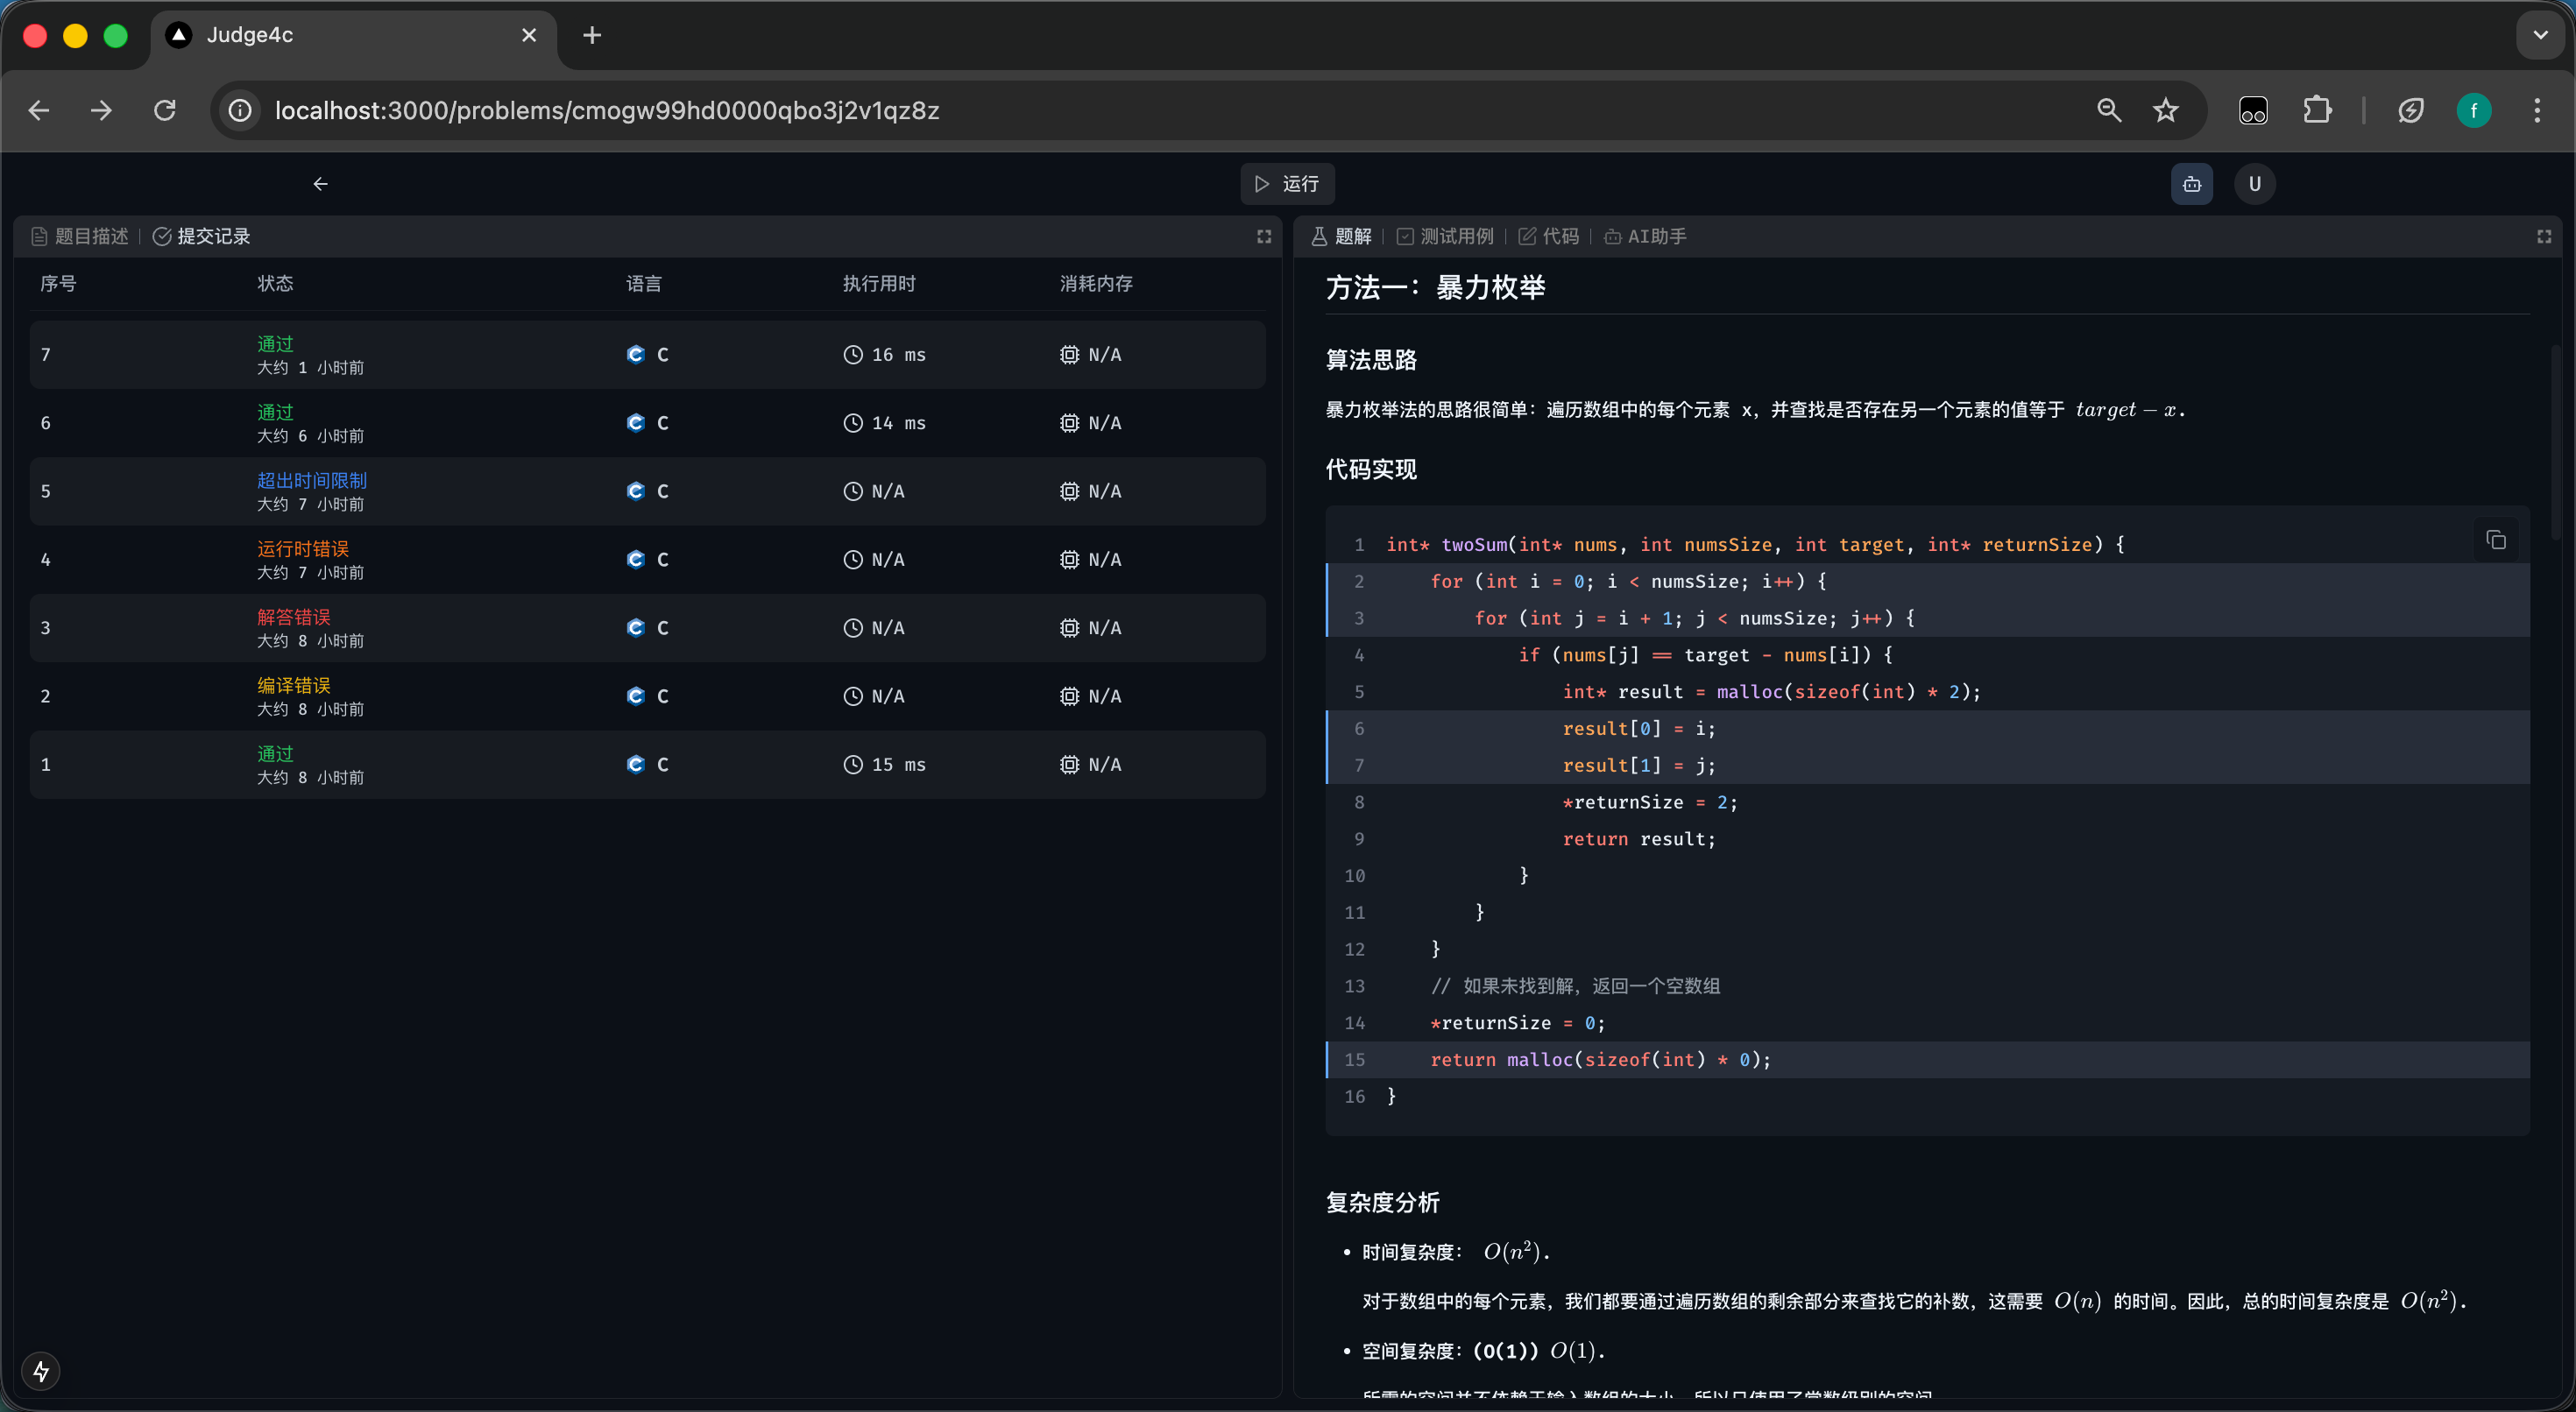
\includegraphics[width=0.96\textwidth]{images/fig6-6.png}
  \caption{深色主题下的题目工作区截图}
  \label{fig:dark-theme-workspace}
\end{figure}

\begin{figure}[htbp]
  \centering
  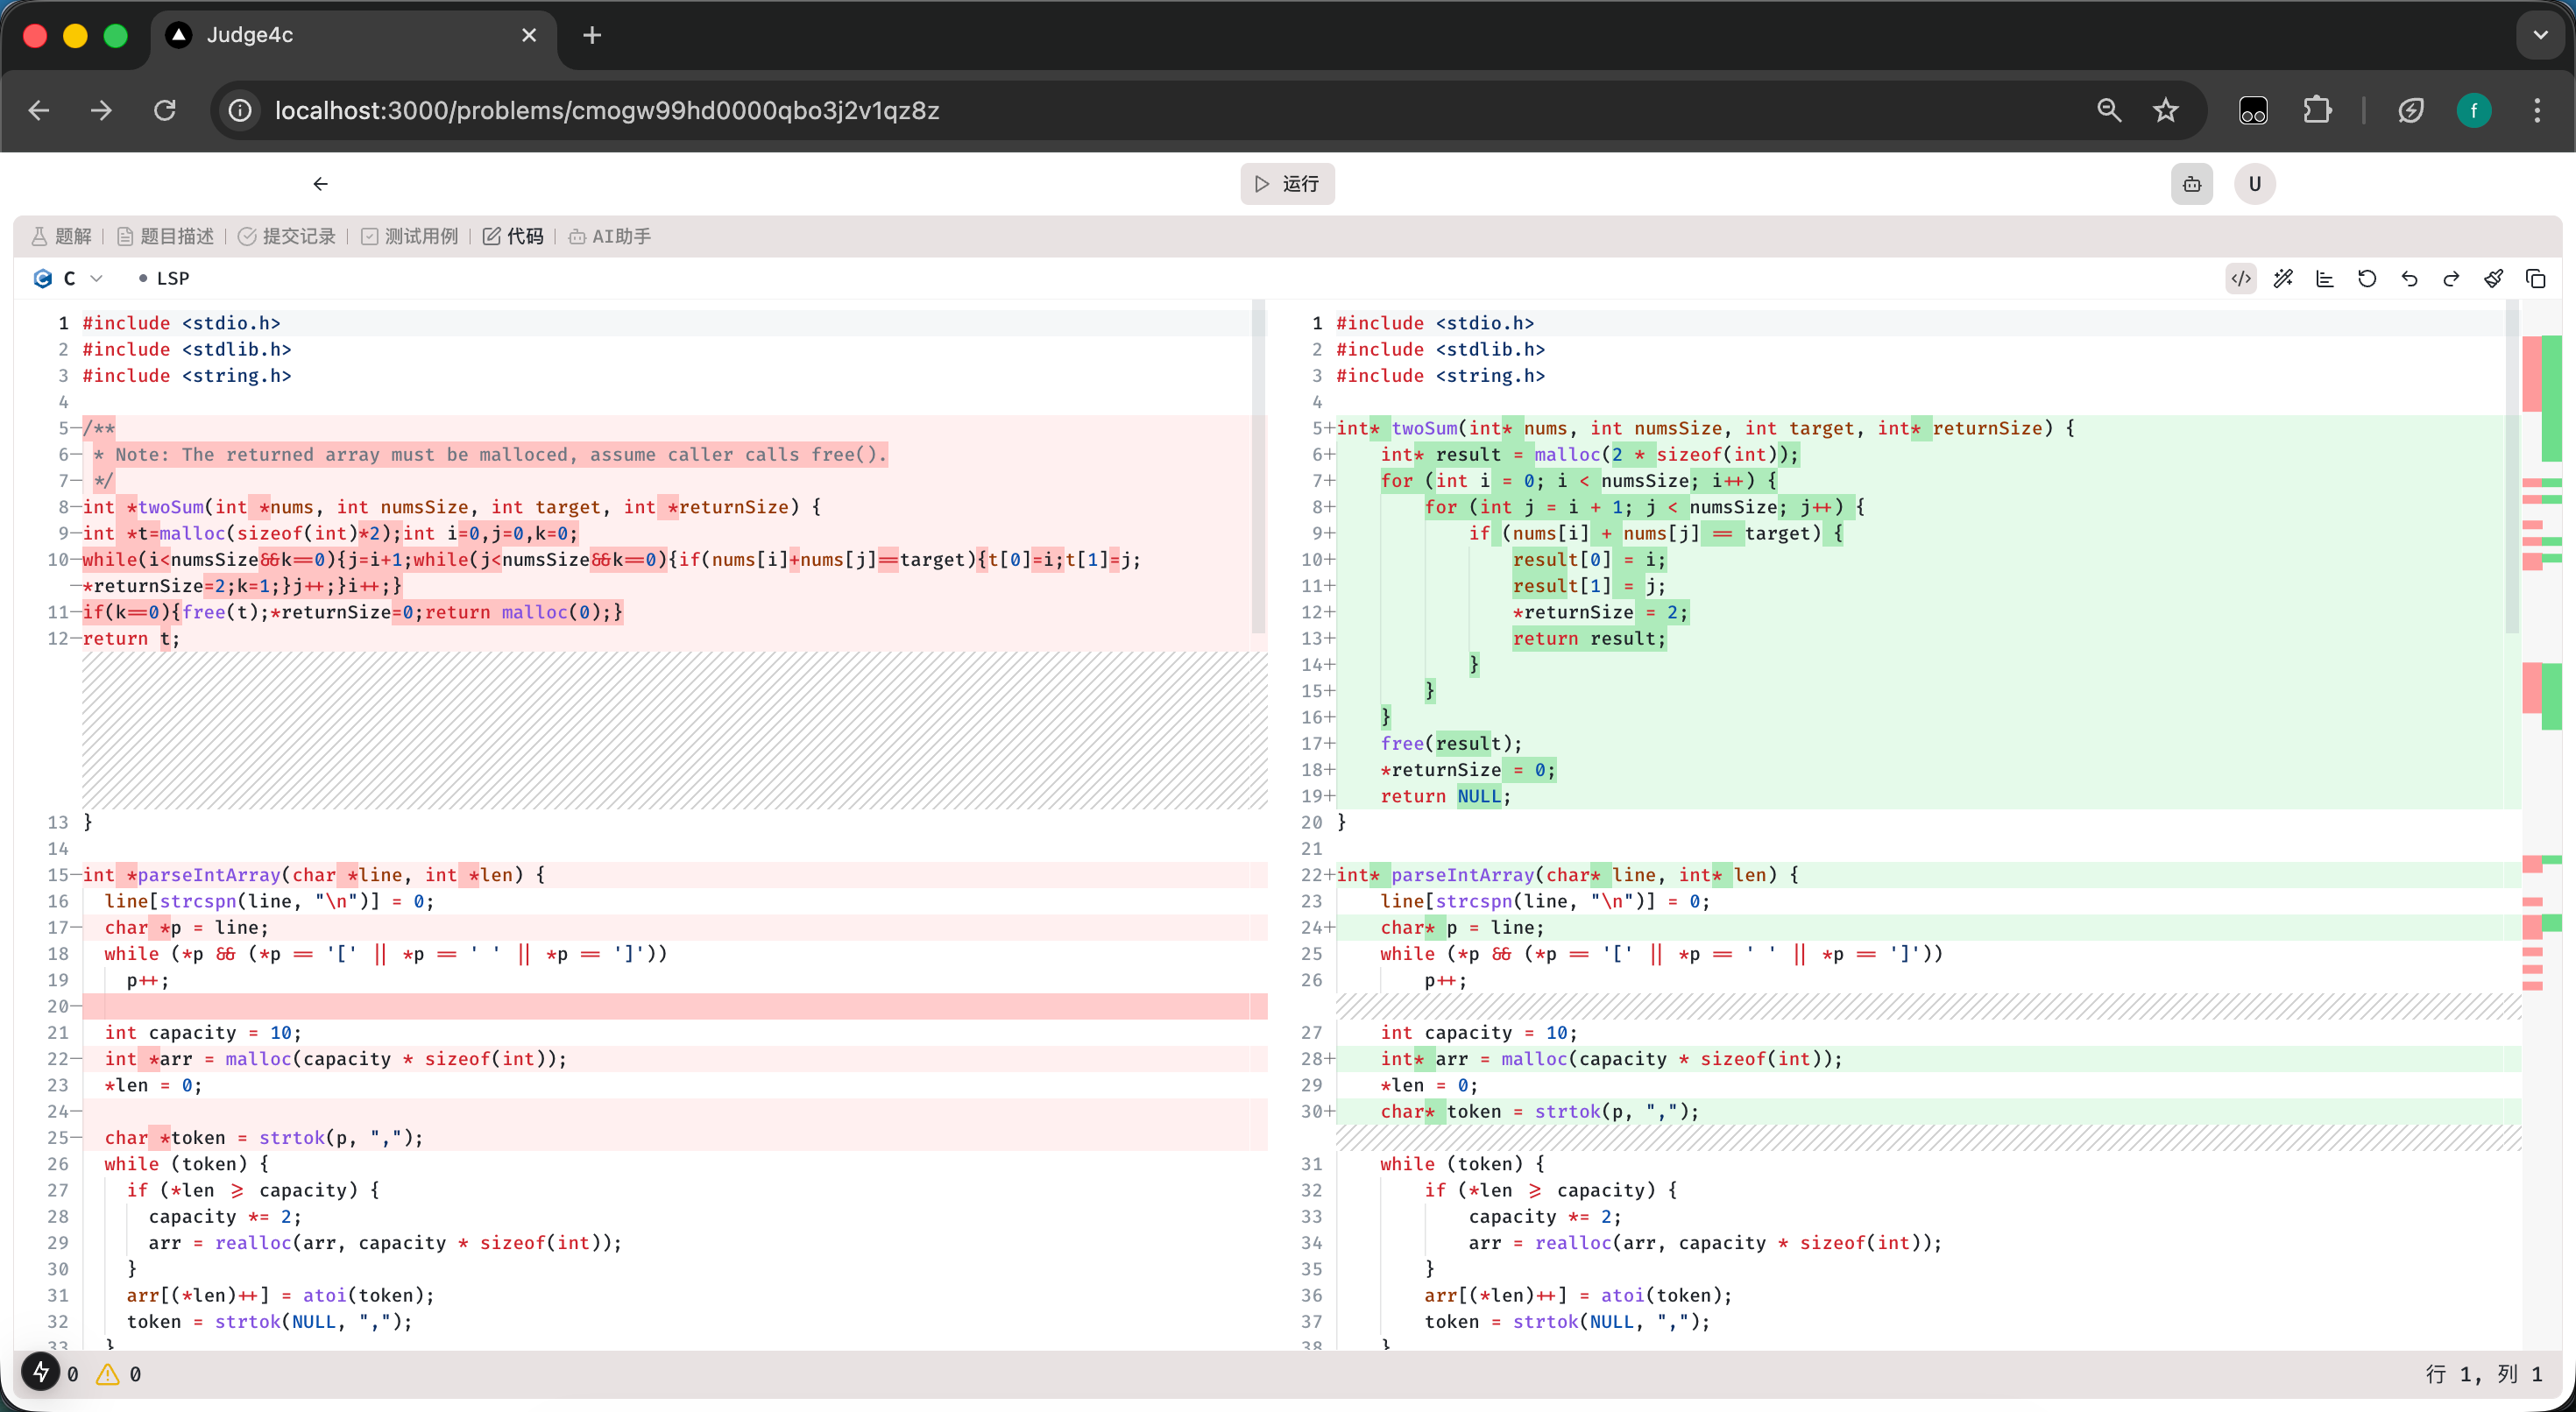
\includegraphics[width=0.96\textwidth]{images/fig6-7.png}
  \caption{优化代码后的 Diff 对比视图截图}
  \label{fig:diff-view}
\end{figure}

\begin{figure}[htbp]
  \centering
  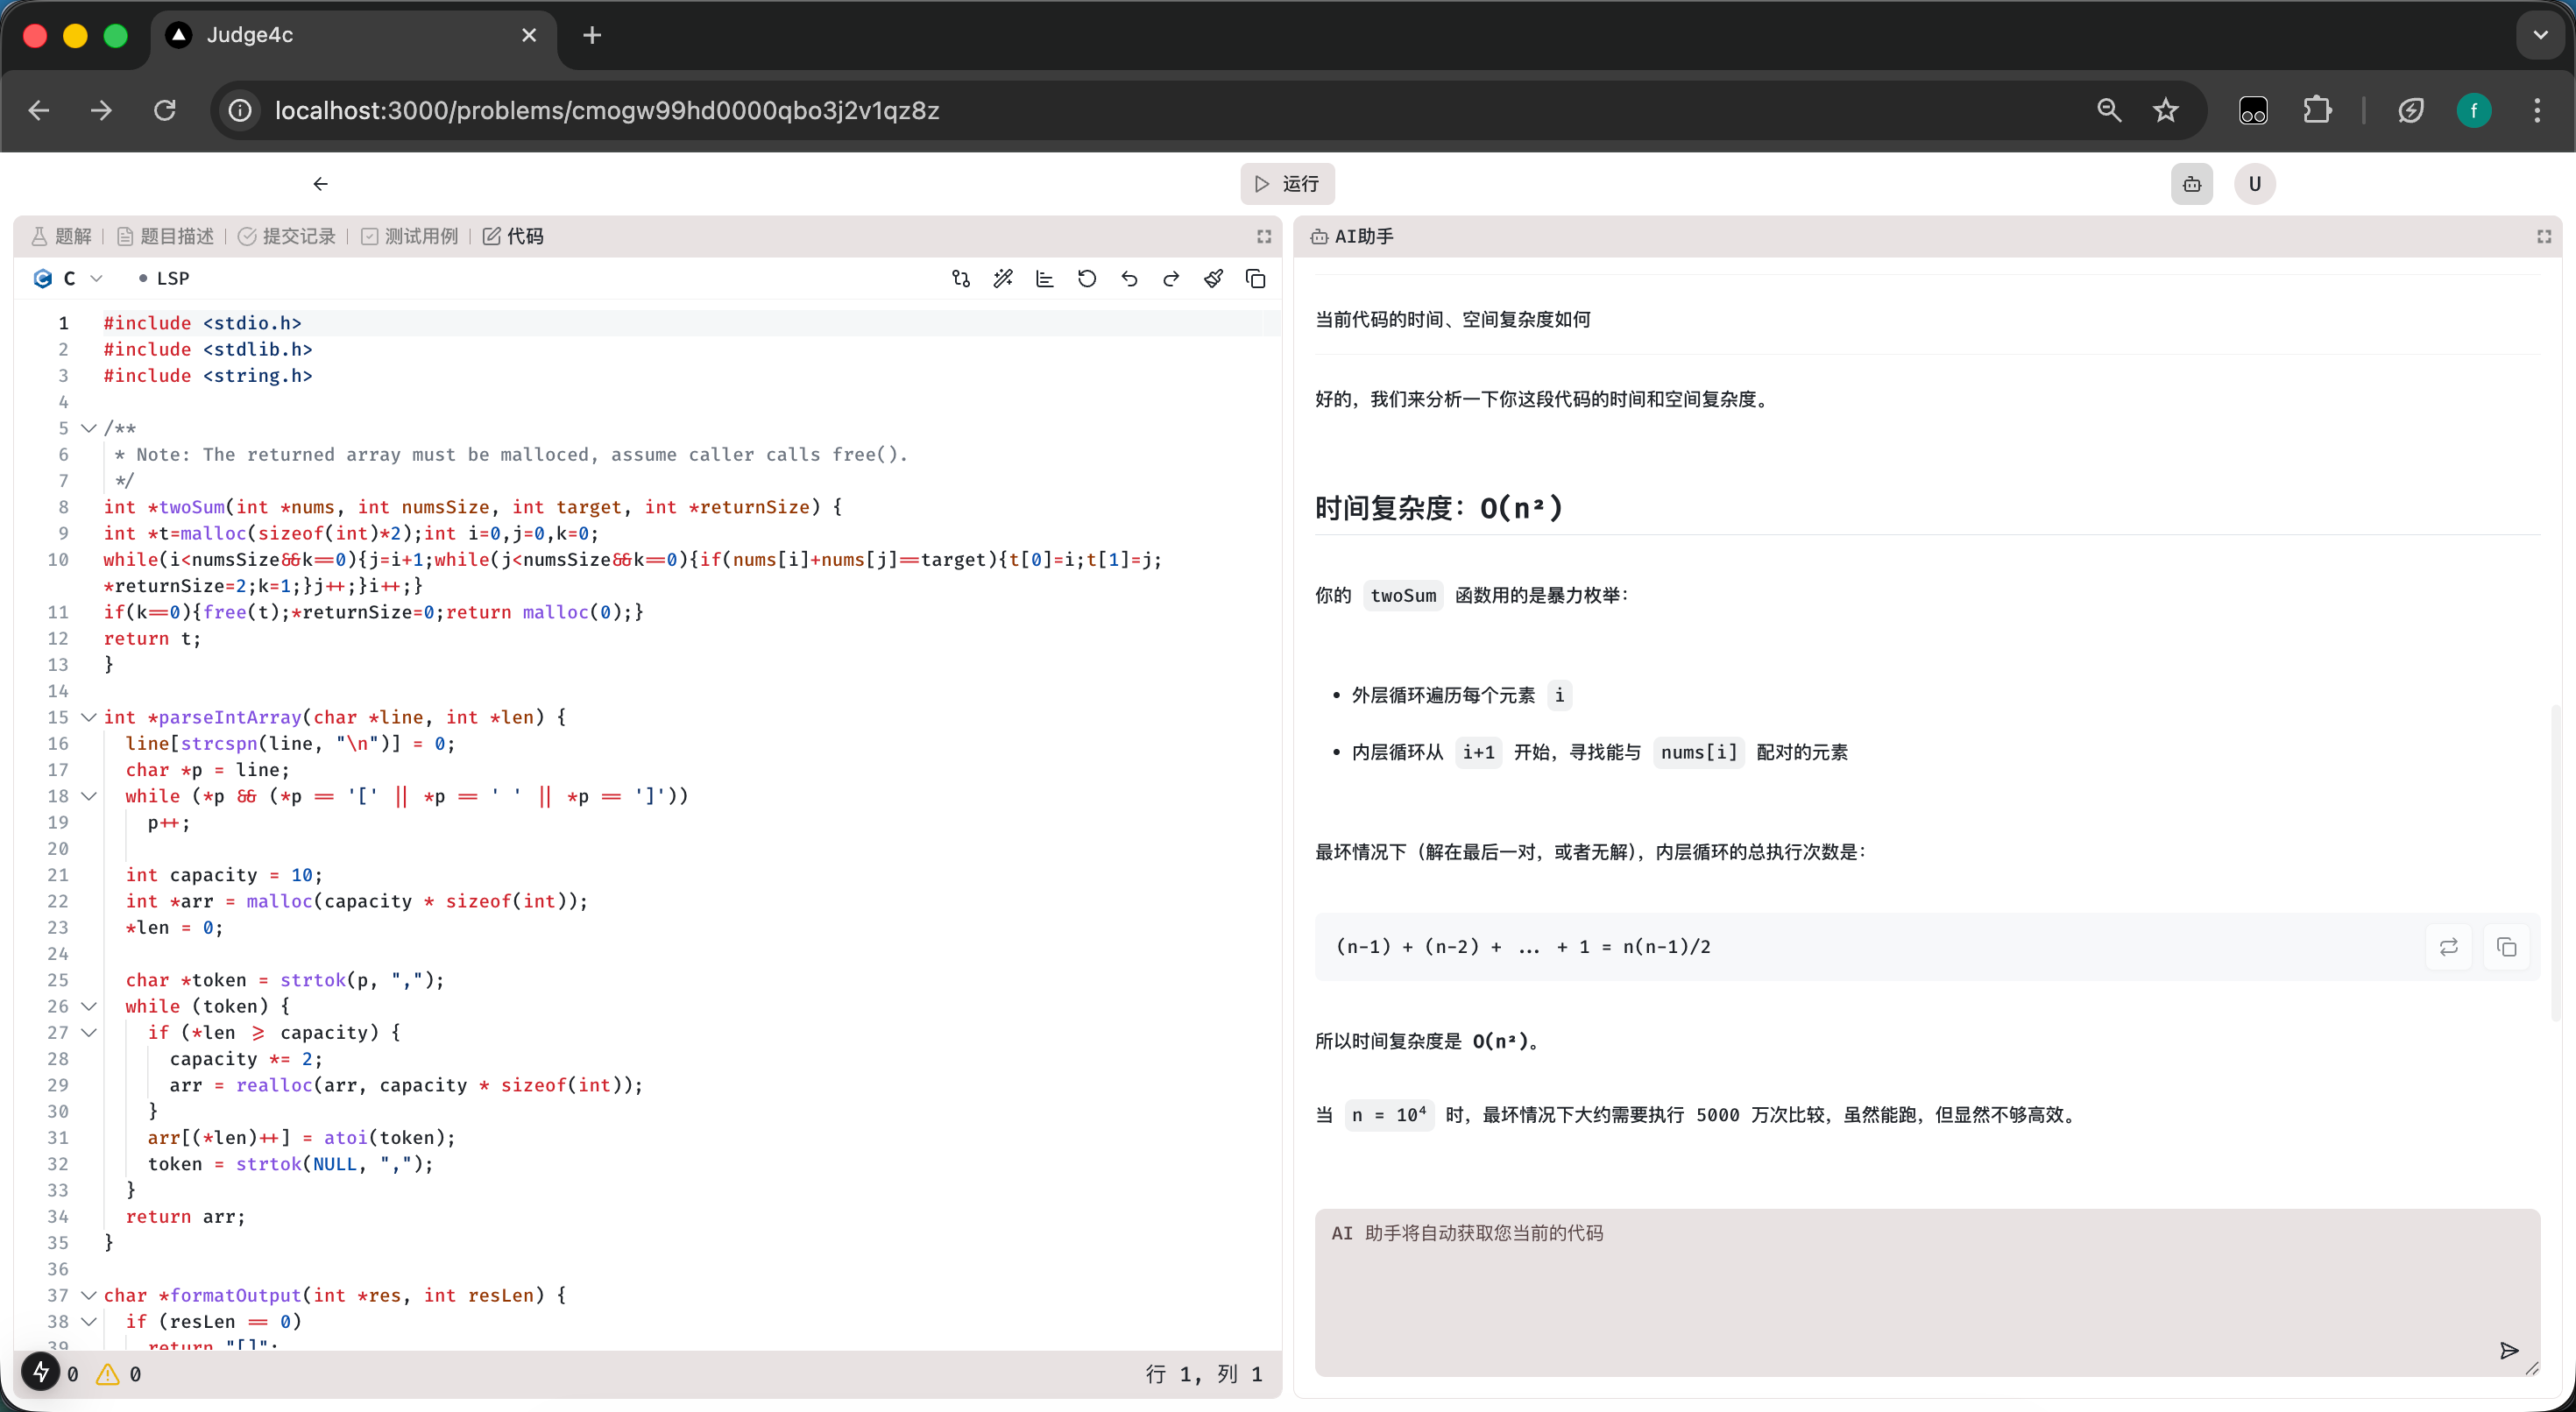
\includegraphics[width=0.96\textwidth]{images/fig6-8.png}
  \caption{AI 助手面板问答截图}
  \label{fig:ai-chat-panel}
\end{figure}

\FloatBarrier
\section{本章小结}

本章给出了测试环境、核心功能、判题正确性、AI 反馈及界面交互的结果。结合正文截图和附录样例代码可见，该系统已经具备可演示、可复核的运行基础，系统核心流程已经跑通，基础判题状态识别基本准确，AI 反馈能够作为补充解释使用。

\chapter{总结与展望}

\section{工作总结}

本文围绕“基于云原生与AI辅助的一体化在线编程评测平台设计与实现”这一课题，完成了需求分析、总体设计、详细实现与测试分析，形成了面向高校程序设计教学场景的在线评测平台原型。论文的主线目标是把客观判题、容器化执行和 AI 辅助反馈整合到同一平台中。

在实现层面，平台已完成题库管理、题目展示、模板加载、在线提交、Docker 隔离编译运行、提交记录展示和 AI 分析等核心功能。第六章的测试结果表明，系统能够正确返回 \texttt{AC}、\texttt{CE}、\texttt{WA}、\texttt{RE}、\texttt{TLE} 等常见状态，前端工作区、多语言切换、主题切换以及编辑阶段 AI 工具也可以正常使用。项目同时通过了 \texttt{bun run lint} 与 \texttt{bun run build} 校验。

除主线功能外，论文还对异步判题、实时状态回传、课程与作业组织、课程级运行环境配置等扩展方向进行了设计论证。这些内容虽然尚未全部进入当前主线实现，但已经为后续继续迭代保留了结构基础。

\section{不足与展望}

当前系统仍有三个直接限制。第一，主线实现主要围绕 C 和 C++，语言覆盖范围有限；第二，判题流程仍以一次提交对应一次容器执行为主，尚未正式切换到独立 worker 与任务队列结合的异步模式；第三，课程、作业和课程级运行环境配置仍停留在设计和预留阶段。

AI 辅助部分也还有改进空间。当前系统已经能够提供复杂度分析、代码优化建议和问答支持，但在反馈稳定性、教师侧审阅、边界控制和更细粒度学习提示方面还不够完善。后续若继续迭代，可优先补充反馈分级、异常内容过滤以及教师侧摘要能力。

若按更高研究标准要求，本文尚未展开并发提交时延、基础设施成本、环境影响、视觉反馈和学生自编测试评价等实验。这些内容在相关研究中具有独立价值[16-18]，也是当前论文与硕博层面工作之间的主要差距。

从后续实现优先级看，应先补齐课程与作业组织能力、课程级运行环境配置以及异步判题主线；排行榜等展示型功能可以后置；竞赛模块则更适合作为后续独立方向，不宜继续挤占当前毕设主线。

\backmatter
\begin{acknowledgements}

本文在课题选定、系统实现、论文撰写和材料整理过程中，得到了许多老师、同学和家人的关心与帮助。在此，谨向在毕业设计期间给予我指导和支持的各位老师表示诚挚的感谢。指导教师在研究方向确定、系统方案设计、论文结构安排以及写作规范把握等方面提供了耐心细致的指导，使本文能够较为顺利地完成。

同时，感谢学院各位任课教师在程序设计、软件工程、数据库与云原生相关课程中的教学与培养，为本课题的完成奠定了理论与实践基础；感谢在项目调试、功能验证和论文修改过程中给予帮助的同学与朋友；感谢家人在学习和生活上的理解与支持。本文还参考了相关开源项目、技术文档与研究成果，在此一并致谢。由于本人水平有限，论文和系统实现中仍难免存在不足之处，恳请各位老师和读者批评指正。

\end{acknowledgements}

\begin{bibprint}
\nocite{*}
\printbibliography[heading=none]
\end{bibprint}

\begin{appendices}

\section{判题测试样例代码}
\pdfbookmark[1]{附录1 判题测试样例代码}{appendix:testcases}

本附录汇总第六章判题正确性测试与 AI 辅助反馈测试所使用的 C 语言样例代码。相关样例支撑了图5-5、图5-6、图5-7、图6-1、图6-3以及表6-3、表6-4、表6-5中的实验说明。

本文实验通过以下命令完成依赖生成、数据初始化与构建校验：

\begin{verbatim}
bunx prisma generate
bunx prisma db seed
bun run build
\end{verbatim}

统一测试题目为“1000 两数之和”，统一测试语言为 C，统一做法为保留系统默认模板，只替换 \texttt{twoSum(...)} 函数。

其中，\texttt{AC}、\texttt{CE}、\texttt{WA}、\texttt{RE}、\texttt{TLE} 五类样例主要用于支撑判题正确性测试；低效正确样例用于展示复杂度分析与优化建议；可读性较差但可通过样例用于展示代码风格与可读性评价能力。

\subsection*{AC 样例}
预期状态为 AC；该样例也可作为“低效正确代码”用于 AI 复杂度分析。

\begin{verbatim}
int *twoSum(int *nums, int numsSize, int target, int *returnSize) {
  for (int i = 0; i < numsSize; i++) {
    for (int j = i + 1; j < numsSize; j++) {
      if (nums[i] + nums[j] == target) {
        int *res = malloc(sizeof(int) * 2);
        res[0] = i;
        res[1] = j;
        *returnSize = 2;
        return res;
      }
    }
  }

  *returnSize = 0;
  return malloc(0);
}
\end{verbatim}

\subsection*{CE 样例}
预期状态为 CE；适合展示系统编译报错能力以及 AI 对语法错误的解释能力。

\begin{verbatim}
int *twoSum(int *nums, int numsSize, int target, int *returnSize) {
  int *res = malloc(sizeof(int) * 2)
  res[0] = 0;
  res[1] = 1;
  *returnSize = 2;
  return res;
}
\end{verbatim}

\subsection*{WA 样例}
预期状态为 WA；适合展示系统基于标准输出比对进行判题的能力。

\begin{verbatim}
int *twoSum(int *nums, int numsSize, int target, int *returnSize) {
  int *res = malloc(sizeof(int) * 2);
  res[0] = 0;
  res[1] = 0;
  *returnSize = 2;
  return res;
}
\end{verbatim}

\subsection*{RE 样例}
预期状态为 RE；适合展示系统对运行期异常的识别能力。

\begin{verbatim}
int *twoSum(int *nums, int numsSize, int target, int *returnSize) {
  abort();
}
\end{verbatim}

\subsection*{TLE 样例}
预期状态为 TLE；适合展示系统时间限制控制是否生效。

\begin{verbatim}
int *twoSum(int *nums, int numsSize, int target, int *returnSize) {
  while (1) {
  }
}
\end{verbatim}

\subsection*{可读性较差但可通过样例}
预期状态为 AC；适合用于表6-5中的风格与可读性反馈案例。

\begin{verbatim}
int *twoSum(int *a, int n, int t, int *r) {
  int i = 0;
  for (; i < n; i++) {
    int j = i + 1;
    for (; j < n; j++) {
      if (a[i] + a[j] == t) {
        int *x = malloc(sizeof(int) * 2);
        x[0] = i;
        x[1] = j;
        *r = 2;
        return x;
      }
    }
  }
  *r = 0;
  return malloc(0);
}
\end{verbatim}

\end{appendices}

\end{document}
